\documentclass[11pt,oneside]{article}

\usepackage[T1]{fontenc}
\usepackage[utf8]{inputenc}
\IfFileExists{libertinus.sty}{\usepackage{libertinus}}{\usepackage{lmodern}}
\usepackage{microtype}
\usepackage[a4paper,margin=27mm,headheight=14pt]{geometry}
\usepackage{amsmath,amssymb,amsthm,mathtools}
\usepackage{booktabs,longtable,array,tabularx}
\usepackage{enumitem}
\usepackage{graphicx}
\usepackage{float}
\usepackage{xcolor}
\usepackage{hyperref}
\usepackage[nameinlink,capitalise]{cleveref}
\usepackage{fancyhdr}
\usepackage{listings}
\usepackage{caption}
\usepackage{subcaption}
\usepackage{url}

\definecolor{deepblue}{RGB}{28,70,112}
\definecolor{deepgreen}{RGB}{32,112,72}
\definecolor{amber}{RGB}{173,99,0}
\definecolor{deepred}{RGB}{145,40,40}
\definecolor{shade}{RGB}{246,248,250}
\definecolor{rulegray}{RGB}{190,198,205}

\hypersetup{
  colorlinks=true,
  linkcolor=deepblue,
  citecolor=deepgreen,
  urlcolor=deepblue,
  pdftitle={Representation Atlas and New Analytic Bridges for the Fabius and Rvachev Functions},
  pdfauthor={OpenAI GPT-5.6 Pro}
}

\pagestyle{fancy}
\fancyhf{}
\fancyhead[L]{Fabius--Rvachev representation atlas}
\fancyhead[R]{\thepage}
\renewcommand{\headrulewidth}{0.4pt}
\setlength{\headheight}{14pt}
\setlength{\emergencystretch}{3em}
\setcounter{tocdepth}{2}
\setcounter{secnumdepth}{3}

\newtheorem{theorem}{Theorem}[section]
\newtheorem{proposition}[theorem]{Proposition}
\newtheorem{lemma}[theorem]{Lemma}
\newtheorem{corollary}[theorem]{Corollary}
\newtheorem{conjecture}[theorem]{Conjecture}
\newtheorem{problem}[theorem]{Problem}
\theoremstyle{definition}
\newtheorem{definition}[theorem]{Definition}
\newtheorem{example}[theorem]{Example}
\theoremstyle{remark}
\newtheorem{remark}[theorem]{Remark}
\newtheorem{warning}[theorem]{Warning}

\newcommand{\R}{\mathbb R}
\newcommand{\C}{\mathbb C}
\newcommand{\N}{\mathbb N}
\newcommand{\Z}{\mathbb Z}
\newcommand{\E}{\mathbb E}
\newcommand{\Prob}{\mathbb P}
\newcommand{\Up}{\operatorname{up}}
\newcommand{\sinc}{\operatorname{sinc}}
\newcommand{\e}{\mathrm e}
\newcommand{\ii}{\mathrm i}
\newcommand{\dd}{\,\mathrm d}
\newcommand{\pv}{\operatorname{pv}}
\newcommand{\supp}{\operatorname{supp}}
\newcommand{\Var}{\operatorname{Var}}
\newcommand{\Cov}{\operatorname{Cov}}
\newcommand{\Law}{\operatorname{Law}}
\newcommand{\dist}{\mathrel{\stackrel{\mathrm d}=}}
\newcommand{\bigO}{\mathcal O}
\newcommand{\smallo}{o}
\newcommand{\vtwo}{v_2}
\newcommand{\wt}{s_2}
\newcommand{\floor}[1]{\left\lfloor #1\right\rfloor}
\newcommand{\ceil}[1]{\left\lceil #1\right\rceil}
\newcommand{\qbinom}[3]{\genfrac{[}{]}{0pt}{}{#1}{#2}_{#3}}
\newcommand{\pospart}[1]{\left(#1\right)_{+}}
\newcommand{\GammaDy}{\Gamma_{\!\mathrm{dy}}}
\newcommand{\GammaGeom}{\Gamma_{\langle q\rangle}}
\newcommand{\Acal}{\mathcal A}
\newcommand{\Fcal}{\mathcal F}
\newcommand{\Repo}{\textcolor{deepblue}{\textbf{[repository]}}}
\newcommand{\Derived}{\textcolor{deepgreen}{\textbf{[derived synthesis]}}}
\newcommand{\New}{\textcolor{amber}{\textbf{[proved here]}}}
\newcommand{\Conj}{\textcolor{deepred}{\textbf{[conjecture]}}}
\newcommand{\RepoShort}{\textcolor{deepblue}{\textbf{[repo]}}}
\newcommand{\DerivedShort}{\textcolor{deepgreen}{\textbf{[derived]}}}
\newcommand{\NewShort}{\textcolor{amber}{\textbf{[new]}}}
\newcommand{\CommitID}{\texttt{0770442945d65bac5530\allowbreak c4f214c6c52c4cb9fbdc}}

\newenvironment{resultbox}{%
  \par\medskip\noindent\begin{center}\begin{minipage}{0.94\textwidth}%
  \color{black}\hrule\vspace{0.65em}\small
}{%
  \vspace{0.65em}\hrule\end{minipage}\end{center}\medskip
}

\lstdefinestyle{pythonstyle}{
  language=Python,
  basicstyle=\ttfamily\small,
  backgroundcolor=\color{shade},
  frame=single,
  rulecolor=\color{rulegray},
  columns=fullflexible,
  keepspaces=true,
  showstringspaces=false,
  breaklines=true,
  xleftmargin=0.5em,
  xrightmargin=0.5em
}

\title{\bfseries Representation Atlas and New Analytic Bridges\\[0.35em]
\Large for the Fabius Function, Rvachev's Up-Function,\\
and Their Fourier Images}
\author{Research report prepared by OpenAI GPT-5.6 Pro\\
\small Source audit: Vladimir Reshetnikov's \texttt{ProveIt} repository}
\date{27 August 2026}

\begin{document}
\maketitle

\begin{abstract}
This report gives a source-audited atlas of integral, series, product, convolution,
probabilistic, spectral, and transform representations of the bounded Fabius function
$F$, Rvachev's compactly supported even function $\Up$, the inverse Fabius function
$Q=F^{-1}$, and the entire Fourier image
\(
 \Phi(z)=\widehat\Up(z).
\)
The baseline material is organized from the current formal exposition and the living
non-formalized frontier documents in the \texttt{ProveIt} repository.  Previously present
results -- including the sinc and cosine products, the arithmetic canonical product,
Fredholm determinants, half-integer spectral series, $q$-binomial moment formulae,
Thue--Morse splines, the generalized-gamma-convolution dual, and the logistic dual -- are
explicitly quarantined from novelty claims.

Five new-to-the-audited-corpus theorem packages are developed.  First, a meromorphic
\emph{dyadic gamma function}
\[
 \Gamma_{\!\mathrm{dy}}(z)=\prod_{h\ge0}\Gamma(1+2^{-h}z)
\]
factors the Rvachev transform as
\(
 \Phi(z)=\bigl(\Gamma_{\!\mathrm{dy}}(z)
 \Gamma_{\!\mathrm{dy}}(-z)\bigr)^{-1}
\), with functional equations, canonical products, digamma and heat-trace integrals, and a
geometric-$q$ extension.  Second, the existing dyadic logistic series is identified in law
with an explicit Gaussian variance mixture driven by the existing discrete Thorin random
variable; this yields a convolution semigroup, a closed Levy density, complete monotonicity
of the density as a function of $x^2$, and dimension-free radial positive definiteness.
Third, Jensen's circular mean of $\log|\Phi|$ is evaluated exactly by binary digit sums and a
finite factorial product.  Fourth, the unbounded zero multiplicities prove that $\Phi$ is
not D-finite, and neither are the dyadic gamma factors.  Fifth, distributional and compact
Fourier formulae for $F$ are completed by an odd-harmonic sine series, while $Q$ receives a
new nonlinear Fourier transform and sine-series representation in terms of oscillatory
integrals of $F$.

A fully commented Python program independently checks the principal identities, produces
four figures, and records truncation diagnostics.  ``Proved here'' means proved in this
report and not found by targeted collision searches in the audited repository; it is not a
claim of priority over all external literature.
\end{abstract}

\tableofcontents
\clearpage

\section{Scope, source audit, and status discipline}
\label{sec:audit}

\subsection{Repository boundary}

The requested source boundary was the recursive collection of \texttt{*.tex} files below
\begin{center}
\small
\url{https://github.com/VladimirReshetnikov/ProveIt/tree/main/Analysis/FabiusFunction/docs}.
\end{center}
The primary formal exposition was pinned to repository commit
\CommitID, dated 27 August 2026.  During the audit the
branch changed: in particular, a support-free quantile substitution theorem entered the
primary exposition.  Consequently, quantile pushforward formulae that looked new against an
earlier snapshot are classified here as repository consequences, not new results.

The recursive audit included the current formal exposition, the consolidated frontier
notebook, the glossary and Lean walkthrough, the active frontier directories, the embedded
literature sources, and the archive provenance map.  The active frontier root contained
seventeen named draft packages at the time of the audit.  One of those packages records a
snapshot with sixty-seven distinct TeX paths.  Historical byte-identical copies were not
counted as independent mathematical sources: the archive provenance file was used to map
them to their living successors, after which the successor source was audited at formula
level.  This avoids manufacturing ``novelty'' merely by overlooking a renamed or moved draft.

\subsection{Collision quarantine}

The following structures were already present and are therefore baseline in this report:
\begin{itemize}[leftmargin=2em]
\item the infinite sinc product, weighted cosine product, and integer-zero canonical product;
\item the arithmetic multiplicities $a_n=1+\vtwo(n)$, their Dirichlet series, counting law
      $\sum_{n\le N}a_n=2N-\wt(N)$, lobe signs, heat traces, spectral zeta functions, and
      Fredholm determinant;
\item half-integer cosine expansions, spectral quadrature, sampling and alias formulae;
\item moments and cumulants through Bell and Bernoulli numbers, $q$-binomial and multiple-zeta
      formulae, Appell sequences, Barnes-type prefixes, and Thue--Morse finite blocks;
\item the discrete-Thorin generalized gamma convolution
      $\E\e^{-wV_\tau}=\Acal(w)^{-\tau}$ and its complete-Bernstein/Stieltjes consequences;
\item the dyadic logistic series whose characteristic function is the reciprocal moment
      generating function of the compact Rvachev law;
\item exact negative-Laplace decompositions, periodic lower-Lambert endpoint asymptotics,
      inverse asymptotics, and the now-formal quantile substitution theorem.
\end{itemize}
Targeted searches did not find the phrases or exact structures ``dyadic gamma'', ``Gaussian
variance mixture'', ``Jensen circular mean'', ``D-finite'', the principal-value transform
of the global Fabius CDF, or the inverse sine coefficients derived in
\cref{sec:inverse-fourier}.  These results are marked \New.  Formulae obtained by combining
known repository theorems without a substantively new bridge are marked \Derived.

\subsection{Status legend and limits of the novelty statement}

\begin{longtable}{@{}p{0.18\textwidth}p{0.75\textwidth}@{}}
\toprule
Status & Meaning \\
\midrule
\endhead
\Repo & Present in the formal exposition or an audited frontier document. \\
\Derived & A direct synthesis or reformulation of repository results; no novelty claim. \\
\New & Proved in this report and not located by targeted collision searches in the audited
       corpus.  This is a corpus-relative statement, not universal priority. \\
\Conj & A plausible but unproved statement, separated from theorems. \\
\bottomrule
\end{longtable}

\section{Normalization and the master probability diagram}
\label{sec:normalization}

\subsection{The compact law and its CDF}

Let $(V_j)_{j\ge1}$ be independent uniform random variables on $[0,1]$, let
$U_j=2V_j-1$ be uniform on $[-1,1]$, and define
\begin{equation}
 X=\sum_{j\ge1}2^{-j}V_j,
 \qquad
 Y=2X-1=\sum_{j\ge1}2^{-j}U_j.                       \label{eq:XY}
\end{equation}
Then $X\in[0,1]$, $Y\in[-1,1]$, $X\dist1-X$, and $Y\dist-Y$.  The bounded Fabius
function and Rvachev density are
\begin{equation}
 F(x)=\Prob(X\le x),
 \qquad
 \Prob(Y\in\dd y)=\Up(y)\dd y.                       \label{eq:F-up-law}
\end{equation}
The normalizations used below are
\begin{equation}
 \Up(y)=
 \begin{cases}
 F(y+1),&-1\le y\le0,\\
 F(1-y)=1-F(y),&0\le y\le1,\\
 0,&|y|>1,
 \end{cases}                                           \label{eq:F-up-link}
\end{equation}
and
\begin{equation}
 F'(x)=2\Up(2x-1)\qquad(0<x<1).                         \label{eq:Fprime-up}
\end{equation}
Thus $\Up$ is even, nonnegative, $C^\infty$, supported on $[-1,1]$, and has integral one.
The density of $X$ is $f_X(x)=2\Up(2x-1)$ on $[0,1]$.

\subsection{Fixed-point integral equations}

The random affine fixed point
\begin{equation}
 Y\dist\frac{U+Y'}2,                                    \label{eq:random-fixed}
\end{equation}
where $U$ is uniform on $[-1,1]$ and $Y'$ is an independent copy of $Y$, gives the exact
refinement equation
\begin{equation}
 \boxed{\quad
 \Up(x)=\int_{2x-1}^{2x+1}\Up(t)\dd t.
 \quad}                                                  \label{eq:up-integral-refinement}
\end{equation}
Differentiation gives
\begin{equation}
 \Up'(x)=2\Up(2x+1)-2\Up(2x-1).                         \label{eq:up-differential-refinement}
\end{equation}
The bounded Fabius function is the fixed point of
\begin{equation}
 F(x)=
 \begin{cases}
 \displaystyle\int_0^{2x}F(t)\dd t,&0\le x\le\tfrac12,\\[1ex]
 \displaystyle1-\int_0^{2-2x}F(t)\dd t,&\tfrac12\le x\le1,
 \end{cases}                                            \label{eq:F-fixed}
\end{equation}
with constant continuation outside $[0,1]$.  Hence
\begin{equation}
 F'(x)=
 \begin{cases}
 2F(2x),&0<x<\tfrac12,\\
 2F(2-2x),&\tfrac12<x<1.
 \end{cases}                                            \label{eq:F-diffeq-pieces}
\end{equation}
These integral equations are often the most efficient starting point for exact quadrature,
monotonicity, and contraction arguments.

\subsection{The signed global extension and derivative tower}

The repository's signed global extension $\Fcal$ satisfies
\begin{equation}
 \Fcal'(x)=2\Fcal(2x),                                   \label{eq:global-diffeq}
\end{equation}
so iteration gives the all-order identity
\begin{equation}
 \boxed{\quad
 \Fcal^{(m)}(x)=2^{\binom{m+1}{2}}\Fcal(2^m x).
 \quad}                                                  \label{eq:global-derivative-tower}
\end{equation}
After the appropriate unit translation, this yields
\begin{equation}
 \Up^{(m)}(x)=2^{\binom{m+1}{2}}\Fcal(2^m(x+1)).         \label{eq:up-derivative-tower}
\end{equation}
Thus every derivative representation of $\Fcal$ immediately becomes one for $\Up$, and
vice versa.  It is important not to apply \eqref{eq:global-diffeq} directly to the bounded
CDF outside its valid normalization.

\section{Infinite convolutions, finite splines, and head--tail representations}
\label{sec:convolution}

\subsection{Box convolution}

The density of $2^{-j}U_j$ is $2^{j-1}\mathbf1_{[-2^{-j},2^{-j}]}$.  Therefore
\begin{equation}
 \boxed{\quad
 \Up=\mathop{\ast}_{j=1}^{\infty}
 \left(2^{j-1}\mathbf1_{[-2^{-j},2^{-j}]}\right).
 \quad}                                                  \label{eq:infinite-box-convolution}
\end{equation}
This identity may be read in probability, in $L^1$, or through uniform convergence of
successive compact splines.  It directly explains positivity, compact support, smoothness,
and the sinc product of \cref{sec:fourier-atlas}.

Let
\begin{equation}
 Y_N=\sum_{j=1}^N2^{-j}U_j,
 \qquad
 u_N=\mathop{\ast}_{j=1}^{N}
 \left(2^{j-1}\mathbf1_{[-2^{-j},2^{-j}]}\right).        \label{eq:finite-box-spline}
\end{equation}
Then $u_N$ is a piecewise polynomial of degree $N-1$ and
\begin{equation}
 Y=Y_N+2^{-N}Y',
 \qquad
 \Up=u_N\ast\left(2^N\Up(2^N\,\cdot)\right).           \label{eq:head-tail-up}
\end{equation}
Equivalently,
\begin{equation}
 \Up(x)=\E\left[2^N\Up\bigl(2^N(x-Y_N)\bigr)\right].   \label{eq:head-tail-up-expectation}
\end{equation}
For the CDF,
\begin{equation}
 F(x)=\E\left[
 F\left(2^Nx-\sum_{j=1}^N2^{N-j}V_j\right)
 \right],                                                \label{eq:head-tail-F}
\end{equation}
where the inner $F$ is the bounded, clamped CDF.  Formula \eqref{eq:head-tail-F} is an exact
$N$-dimensional cube integral and a useful recursive numerical scheme.

\subsection{General truncated-power spline}

For positive widths $a_1,\dots,a_N$, the density of
$\sum_{j=1}^Na_jU_j$ is
\begin{equation}
 b_N(x)=\frac{1}{(N-1)!\,2^N\prod_{j=1}^Na_j}
 \sum_{\varepsilon\in\{\pm1\}^N}
 \left(\prod_{j=1}^N\varepsilon_j\right)
 \pospart{x+\sum_{j=1}^N\varepsilon_ja_j}^{N-1}.        \label{eq:general-spline}
\end{equation}
Its CDF is obtained by replacing $(N-1)!$ and the exponent $N-1$ by $N!$ and $N$.
For $a_j=2^{-j}$, binary indexing turns \eqref{eq:general-spline} into the exact
Thue--Morse spline
\begin{equation}
 \boxed{\quad
 u_N(x)=\frac{2^{N(N-1)/2}}{(N-1)!}
 \sum_{k=0}^{2^N-1}(-1)^{\wt(k)}
 \pospart{x+\frac{2^N-1-2k}{2^N}}^{N-1}.
 \quad}                                                  \label{eq:TM-spline}
\end{equation}
The corresponding finite CDF is
\begin{equation}
 U_N(x)=\frac{2^{N(N-1)/2}}{N!}
 \sum_{k=0}^{2^N-1}(-1)^{\wt(k)}
 \pospart{x+\frac{2^N-1-2k}{2^N}}^{N}.                  \label{eq:TM-spline-cdf}
\end{equation}
Prouhet cancellation makes the apparent polynomial tails cancel exactly.  These formulae
simultaneously represent the finite probability law, a compact spline, and a signed
Thue--Morse power sum.

\subsection{Hypercube and section representations}

For bounded measurable $g$,
\begin{equation}
 \int_{-1}^{1}g(y)\Up(y)\dd y
 =\int_{[-1,1]^{\N}}g\left(\sum_{j\ge1}2^{-j}u_j\right)
   \bigotimes_{j\ge1}\frac{\dd u_j}{2}.                 \label{eq:infinite-cube}
\end{equation}
At finite depth this gives a coarea interpretation of $u_N$ as the weighted $(N-1)$-
dimensional volume of the cube section
\(
 \sum_{j=1}^N2^{-j}u_j=x.
\)
The infinite-dimensional expression is often more useful than a closed formula: it converts
integrals against $\Up$ into product quadrature and supports concentration and coupling
arguments.

\section{Fourier-product atlas and spectral representations}
\label{sec:fourier-atlas}

\subsection{Conventions and the three canonical products}

We use
\begin{equation}
 \widehat g(z)=\int_{\R}g(x)\e^{-2\pi\ii xz}\dd x,
 \qquad
 \sinc w=\frac{\sin w}{w},                               \label{eq:FT-convention}
\end{equation}
with the removable value at zero.  Put
\begin{equation}
 \Phi(z)=\widehat\Up(z).                                  \label{eq:Phi-def}
\end{equation}
The repository establishes the entire products
\begin{align}
 \Phi(z)
 &=\prod_{h=0}^{\infty}\sinc\left(\frac{\pi z}{2^h}\right),
                                                               \label{eq:Phi-sinc}\\
 &=\prod_{m=1}^{\infty}\left(\cos\frac{\pi z}{2^m}\right)^m,
                                                               \label{eq:Phi-cos}\\
 &=\prod_{n=1}^{\infty}\left(1-\frac{z^2}{n^2}\right)^{a_n},
 \qquad a_n=1+\vtwo(n).                                  \label{eq:Phi-canonical}
\end{align}
They satisfy the Mahler-type renormalization
\begin{equation}
 \Phi(z)=\sinc(\pi z)\Phi(z/2).                           \label{eq:Phi-scale}
\end{equation}
The zero at every nonzero integer $n$ has exact order $a_{|n|}$.

\subsection{Logarithmic Taylor series and partial fractions}

For $|z|<1$,
\begin{equation}
 \boxed{\quad
 \log\Phi(z)=-\sum_{r\ge1}
 \frac{\zeta(2r)}{r(1-4^{-r})}z^{2r}.
 \quad}                                                  \label{eq:logPhi-series}
\end{equation}
Logarithmic differentiation of the canonical product gives, away from the integer zeros,
\begin{equation}
 \frac{\Phi'(z)}{\Phi(z)}
 =-2z\sum_{n\ge1}\frac{a_n}{n^2-z^2}.                   \label{eq:Phi-logderivative}
\end{equation}
The arithmetic spectrum has Dirichlet generating function
\begin{equation}
 \sum_{n\ge1}\frac{a_n}{n^s}
 =\frac{\zeta(s)}{1-2^{-s}},\qquad \Re s>1,              \label{eq:a-Dirichlet}
\end{equation}
and exact counting function
\begin{equation}
 A(N)=\sum_{n\le N}a_n
 =\sum_{h\ge0}\floor{N/2^h}
 =2N-\wt(N).                                             \label{eq:a-count}
\end{equation}
Thus the zero divisor simultaneously encodes the Riemann zeta function, dyadic valuation,
and binary digit sum.

\subsection{Linear and quadratic heat traces}

Two Lambert/heat kernels occur naturally:
\begin{align}
 L_1(t)&=\sum_{n\ge1}a_n\e^{-nt}
       =\sum_{h\ge0}\frac{1}{\e^{2^ht}-1},               \label{eq:L1}\\
 K(t)&=\sum_{n\ge1}a_n\e^{-n^2t}
       =\sum_{h\ge0}\sum_{m\ge1}\e^{-4^hm^2t}.          \label{eq:Kheat}
\end{align}
Their Mellin transforms are
\begin{align}
 \int_0^\infty L_1(t)t^{s-1}\dd t
 &=\Gamma(s)\frac{\zeta(s)}{1-2^{-s}},&&\Re s>1,
                                                               \label{eq:L1-Mellin}\\
 \int_0^\infty K(t)t^{s-1}\dd t
 &=\Gamma(s)\frac{\zeta(2s)}{1-4^{-s}},&&\Re s>\tfrac12.
                                                               \label{eq:K-Mellin}
\end{align}
The consolidated frontier work develops theta completion and complex-dimension oscillations
for $K$.  The linear kernel $L_1$ will reappear in the dyadic-gamma integral and in the Levy
density of the Gaussian-mixture dual.

\subsection{Frullani--Lambert integral for the Fourier product}

Summing the elementary Frullani identity over the zero divisor gives the mixed
integral/product representation
\begin{equation}
 \boxed{\quad
 \log\Phi(z)
 =-2\int_0^\infty\bigl(\cosh(zt)-1\bigr)L_1(t)\frac{\dd t}{t},
 \qquad |\Re z|<1.
 \quad}                                                  \label{eq:Frullani-Phi}
\end{equation}
In particular, for real $y$,
\begin{equation}
 \log\Phi(\ii y)
 =2\int_0^\infty\bigl(1-\cos(yt)\bigr)L_1(t)\frac{\dd t}{t}.  \label{eq:Phi-imag-integral}
\end{equation}
This writes the Wick-rotated product as the exponential of a positive Lambert-kernel energy.
It is also the Levy--Khintchine exponent that underlies \cref{sec:gaussian-mixture}.

\subsection{Fredholm determinant and spectral zeta}

Let $D$ be the positive diagonal operator whose eigenvalue $n$ occurs with multiplicity
$a_n$.  Since $D^{-2}$ is trace class,
\begin{equation}
 \boxed{\quad
 \Phi(z)=\det(I-z^2D^{-2}).
 \quad}                                                  \label{eq:Fredholm}
\end{equation}
The associated spectral zeta function is
\begin{equation}
 \zeta_D(s)=\operatorname{tr}(D^{-s})
 =\frac{\zeta(s)}{1-2^{-s}},\qquad \Re s>1.              \label{eq:spectral-zeta}
\end{equation}
The determinant, zero multiplicities, heat trace, and arithmetic Dirichlet series are thus
four views of the same spectrum.

\section{Fourier inversion, sampling, and interval series}
\label{sec:fourier-inversion}

\subsection{Whole-line inversion}

Because $\Up\in C_c^\infty(\R)$, its transform is rapidly decreasing on the real axis and
\begin{align}
 \Up(x)
 &=\int_{\R}\Phi(\xi)\e^{2\pi\ii x\xi}\dd\xi,           \label{eq:up-inversion}\\
 &=2\int_0^\infty\Phi(\xi)\cos(2\pi x\xi)\dd\xi.       \label{eq:up-cos-integral}
\end{align}
Every derivative may be obtained under the integral:
\begin{equation}
 \Up^{(m)}(x)=\int_{\R}(2\pi\ii\xi)^m
 \Phi(\xi)\e^{2\pi\ii x\xi}\dd\xi.                   \label{eq:up-derivative-Fourier}
\end{equation}
Combining this with \eqref{eq:Phi-sinc}, \eqref{eq:Phi-canonical}, or the dyadic-gamma
factorization below gives distinct integral--product representations of the same bump.

\subsection{Poisson partition and half-integer spectrum}

The integer zeros imply the partition of unity
\begin{equation}
 \sum_{k\in\Z}\Up(x-k)=1.                                \label{eq:partition-unity}
\end{equation}
On $[-1,1]$, the half-integer samples give the rapidly convergent cosine expansion
\begin{equation}
 \boxed{\quad
 \Up(t)=\frac12+\sum_{k\ge0}
 \Phi\left(k+\frac12\right)
 \cos\bigl((2k+1)\pi t\bigr).
 \quad}                                                  \label{eq:up-half-cosine}
\end{equation}
The active half-integer spectral report develops weighted Prouhet identities, exact alias
transforms, and spectral quadrature from this series.

\subsection{Paley--Wiener sampling of the Fourier image}

Since $\Up$ is supported on $[-1,1]$, $\Phi$ belongs to the Paley--Wiener space of bandwidth
one.  Shannon sampling at spacing $1/2$ gives
\begin{equation}
 \Phi(z)=\sum_{k\in\Z}\Phi(k/2)
 \sinc\bigl(\pi(2z-k)\bigr).                             \label{eq:Phi-Shannon}
\end{equation}
The rapid decay of the samples makes the series locally uniformly and absolutely
convergent.  Since $\Phi(m)=0$ for every nonzero integer $m$,
\begin{equation}
 \Phi(z)=\sinc(2\pi z)+
 \sum_{\substack{k\in\Z\\k\ \mathrm{odd}}}
 \Phi(k/2)\sinc\bigl(\pi(2z-k)\bigr).                   \label{eq:Phi-Shannon-odd}
\end{equation}
Thus the entire transform is reconstructed from its half-integer arithmetic ray.

\subsection{Fourier--Legendre representation}

The compact interval also supports the uniformly convergent Legendre expansion
\begin{equation}
 \Up(x)=\sum_{m\ge0}\frac{2m+1}{2}
 \left(\int_{-1}^1\Up(t)P_m(t)\dd t\right)P_m(x).        \label{eq:Legendre}
\end{equation}
Evenness removes the odd indices.  The coefficient can be expressed either as a moment
combination or by inserting \eqref{eq:up-cos-integral} and using the Fourier--Bessel transform
of $P_m$.  This is a useful bridge between exact moments and orthogonal approximation.

\section{Laplace, Mellin, moment, and \texorpdfstring{$q$}{q}-series representations}
\label{sec:laplace-moments}

\subsection{Moment-generating and Laplace products}

The random series gives the entire moment-generating functions
\begin{align}
 M_Y(t)=\E\e^{tY}
 &=\Phi\left(\frac{\ii t}{2\pi}\right)
 =\prod_{j\ge1}\frac{\sinh(t/2^j)}{t/2^j},               \label{eq:MY}\\
 M_X(t)=\E\e^{tX}
 &=\prod_{j\ge1}\frac{\e^{t/2^j}-1}{t/2^j},             \label{eq:MX}\\
 L_X(s)=\E\e^{-sX}
 &=\prod_{j\ge1}\frac{1-\e^{-s/2^j}}{s/2^j}.           \label{eq:LX}
\end{align}
For $c>0$, the CDF has the Bromwich representation
\begin{equation}
 F(x)=\frac{1}{2\pi\ii}\int_{c-\ii\infty}^{c+\ii\infty}
 \frac{L_X(s)}{s}\e^{sx}\dd s.                          \label{eq:F-Bromwich}
\end{equation}
This contour formula is the natural entrance to the lower-Lambert saddle theory.

\subsection{Mellin moments, including negative orders}

For $\Re\alpha>0$,
\begin{equation}
 \E X^{-\alpha}=\frac{1}{\Gamma(\alpha)}
 \int_0^\infty s^{\alpha-1}L_X(s)\dd s.                 \label{eq:negative-moment-Mellin}
\end{equation}
The endpoint flatness makes every negative moment finite.  For $0<\Re\alpha<1$,
\begin{equation}
 \E X^{\alpha}=\frac{\alpha}{\Gamma(1-\alpha)}
 \int_0^\infty\bigl(1-L_X(s)\bigr)s^{-\alpha-1}\dd s. \label{eq:positive-fractional-moment}
\end{equation}
For integer $m\ge1$, integration by parts gives the survival representation
\begin{equation}
 \E X^m=m\int_0^1x^{m-1}\bigl(1-F(x)\bigr)\dd x
 =m\int_0^1x^{m-1}\Up(x)\dd x.                          \label{eq:moments-survival}
\end{equation}

\subsection{Cumulants, Bernoulli numbers, and Bell polynomials}

From \eqref{eq:logPhi-series}, the nonzero cumulants of $Y$ are
\begin{equation}
 \boxed{\quad
 \kappa_{2r}(Y)
 =\frac{B_{2r}}{2r(1-4^{-r})}
 =(-1)^{r+1}\frac{(2r)!\zeta(2r)}
 {r(1-4^{-r})(2\pi)^{2r}},
 \quad \kappa_{2r+1}(Y)=0.
 \quad}                                                  \label{eq:Y-cumulants}
\end{equation}
Hence
\begin{equation}
 \E Y^{2n}=B_{2n}\bigl(0,\kappa_2,0,\kappa_4,\dots,0,\kappa_{2n}\bigr), \label{eq:Bell-moments}
\end{equation}
where the $B_{2n}$ on the right is the complete exponential Bell polynomial, not a Bernoulli
number.  The first values are
\begin{equation}
 \E Y^2=\frac19,\qquad
 \E Y^4=\frac{19}{675},\qquad
 \E Y^6=\frac{583}{59535}.                               \label{eq:first-moments}
\end{equation}
Moments of $X=(1+Y)/2$ follow by binomial expansion.

\subsection{Wick rotation, Newton recurrence, and \texorpdfstring{$q$}{q}-MZV formula}

Define
\begin{equation}
 \Acal(w)=\Phi(\ii\sqrt w)
 =\prod_{n\ge1}\left(1+\frac{w}{n^2}\right)^{a_n}
 =\sum_{r\ge0}C_rw^r.                                    \label{eq:A-def}
\end{equation}
Then
\begin{equation}
 C_r=\frac{(2\pi)^{2r}}{(2r)!}\E Y^{2r}.                 \label{eq:C-moment}
\end{equation}
Writing
\begin{equation}
 p_r=\sum_{n\ge1}\frac{a_n}{n^{2r}}
 =\frac{\zeta(2r)}{1-4^{-r}},                            \label{eq:pr}
\end{equation}
Newton's recurrence is
\begin{equation}
 rC_r=\sum_{j=1}^r(-1)^{j+1}p_jC_{r-j},\qquad C_0=1.    \label{eq:Newton-C}
\end{equation}
At $q=1/4$, the active frontier report further expands $C_r$ by partitions.  If
$\lambda=(\lambda_1,\dots,\lambda_\ell)\vdash r$, $m_j(\lambda)$ is the multiplicity of
part $j$, and
\begin{equation}
 Z_\lambda=\sum_{\substack{n_1,\dots,n_\ell\ge1\\n_i\ne n_j}}
 \frac{1}{n_1^{2\lambda_1}\cdots n_\ell^{2\lambda_\ell}},                \label{eq:Zlambda}
\end{equation}
then
\begin{equation}
 \boxed{\quad
 C_r=\sum_{\lambda\vdash r}
 \frac{Z_\lambda}{\prod_{j\ge1}m_j(\lambda)!}
 \prod_{i=1}^{\ell(\lambda)}
 \frac{q^{\lambda_i(\lambda_i-1)/2}}{(q;q)_{\lambda_i}},
 \qquad q=\frac14.
 \quad}                                                  \label{eq:q-MZV}
\end{equation}
Moreover $Z_\lambda$ is a symmetrized multiple-zeta value.  This formula keeps both the
integer spectrum and its dyadic layer occupancy visible.

\subsection{Appell and logistic representations already in the corpus}

The Appell sequence associated with the compact Rvachev law is defined by
\begin{equation}
 \frac{\e^{xt}}{M_Y(t)}=\sum_{n\ge0}A_n(x)\frac{t^n}{n!}. \label{eq:Appell}
\end{equation}
The audited Barnes/inverse draft introduces independent standard logistic variables
$\Lambda_j$ and
\begin{equation}
 Z=\sum_{j\ge1}\frac{\Lambda_j}{\pi2^j},                 \label{eq:logistic-Z}
\end{equation}
with
\begin{equation}
 \E\e^{\ii tZ}=\frac{1}{M_Y(t)},
 \qquad
 A_n(x)=\E(x+\ii Z)^n.                                   \label{eq:logistic-dual-baseline}
\end{equation}
This logistic dual is baseline.  The new result in \cref{sec:gaussian-mixture} is its exact
identification as a Gaussian variance mixture driven by the independently developed Thorin
variable.

\section{Thue--Morse, dyadic arithmetic, and finite product-to-sum bridges}
\label{sec:thue-morse}

Let $\varepsilon_k=(-1)^{\wt(k)}$.  The finite Prouhet product is
\begin{equation}
 \prod_{j=0}^{N-1}(1-z^{2^j})
 =\sum_{k=0}^{2^N-1}\varepsilon_kz^k.                    \label{eq:Prouhet-product}
\end{equation}
With $z=\e^t$ this becomes
\begin{equation}
 \sum_{k<2^N}\varepsilon_k\e^{kt}
 =\prod_{j=0}^{N-1}(1-\e^{2^jt}).                         \label{eq:Prouhet-exponential}
\end{equation}
Coefficient comparison yields
\begin{equation}
 \sum_{k<2^N}\varepsilon_kk^m=0\quad(0\le m<N),
 \qquad
 \sum_{k<2^N}\varepsilon_kk^N
 =(-1)^NN!2^{N(N-1)/2}.                                  \label{eq:Prouhet-sharp}
\end{equation}
These cancellations explain the compactness of the truncated-power spline
\eqref{eq:TM-spline}; they also power the exact dyadic-value formulae, Gaussian-binomial
interpolation, and Richardson extrapolants in the repository.

The finite Fourier product
\begin{equation}
 \Phi_N(z)=\prod_{h=0}^{N-1}\sinc\left(\frac{\pi z}{2^h}\right)           \label{eq:PhiN}
\end{equation}
can be converted into a signed exponential sum by expanding the sine factors.  Conversely,
Prouhet cancellations force high-order zeros in those finite sums.  This is the basic
product-to-sum bridge connecting Fourier analysis to exact binary arithmetic.

\section{Endpoint Laplace phases, Lambert \texorpdfstring{$W$}{W}, and inverse asymptotics}
\label{sec:endpoint}

The active frontier synthesis writes
\begin{equation}
 g(s)=\log L_X(s)
 =-\frac{(\log s)^2}{2\log2}+\frac12\log s
   +R(\log_2s)+E(s),                                     \label{eq:g-decomp}
\end{equation}
where $R$ is real-analytic and one-periodic and
\begin{equation}
 0\le E(s)\le\frac{\e^{-s}}{(1-\e^{-s})^2}.              \label{eq:E-bound}
\end{equation}
The CDF integral \eqref{eq:F-Bromwich} has saddle equation
\begin{equation}
 x=-g'(s),                                                \label{eq:saddle-eq}
\end{equation}
whose exact phase is solved by a lower branch of Lambert $W$, perturbed by the periodic
function and its derivatives.  The periodic term is essential: every nonzero Fourier mode is
explicitly nonzero in the formal exposition, so replacing it by a constant loses the claimed
sharp error scale.

The inverse $Q=F^{-1}$ consequently lives on the stretched-logarithmic scale
\begin{equation}
 Q(y)\asymp
 \sqrt{\log(1/y)}
 \exp\left[-\sqrt{2\log2\,\log(1/y)}\right]
 \qquad(y\downarrow0),                                  \label{eq:Q-scale}
\end{equation}
with a sharper periodic Lambert expansion in the audited inverse reports.  Reflection gives
$Q(1-y)=1-Q(y)$.  These asymptotic representations complement, rather than replace, the exact
Fourier and quantile identities developed below.

\clearpage
\part*{New theorem packages}
\addcontentsline{toc}{part}{New theorem packages}

\section{The dyadic gamma factorization}
\label{sec:dyadic-gamma}

\subsection{Definition, convergence, and poles}

\begin{definition}[Dyadic gamma function \New]
For $z\in\C$, away from the negative integers, define
\begin{equation}
 \boxed{\quad
 \GammaDy(z)=\prod_{h=0}^{\infty}\Gamma(1+2^{-h}z).
 \quad}                                                  \label{eq:GammaDy-def}
\end{equation}
\end{definition}

\begin{theorem}[Meromorphy and Mahler equation \New]
The product \eqref{eq:GammaDy-def} converges locally uniformly away from its poles and defines
a meromorphic function satisfying
\begin{equation}
 \GammaDy(z)=\Gamma(1+z)\GammaDy(z/2),
 \qquad \GammaDy(0)=1.                                  \label{eq:GammaDy-Mahler}
\end{equation}
Its pole at $-n$, $n\ge1$, has exact order $a_n=1+\vtwo(n)$ and it has no other poles.
\end{theorem}

\begin{proof}
Uniformly on compact sets, $\log\Gamma(1+w)=-\gamma w+\bigO(w^2)$ as $w\to0$.
The sums $\sum_h2^{-h}$ and $\sum_h4^{-h}$ converge, so the logarithms form a normally
convergent series after finitely many factors are removed.  Separating the factor $h=0$
gives \eqref{eq:GammaDy-Mahler}.  At $z=-n$, the factor indexed by $h$ has a simple gamma
pole precisely when $n/2^h$ is a positive integer, namely for $0\le h\le\vtwo(n)$.  Their
number is $1+\vtwo(n)$.
\end{proof}

\subsection{Reflection factorization of the Rvachev transform}

\begin{theorem}[Dyadic gamma factorization \New]
For every $z\in\C$,
\begin{equation}
 \boxed{\quad
 \Phi(z)=\frac{1}{\GammaDy(z)\GammaDy(-z)}.
 \quad}                                                  \label{eq:Phi-GammaDy}
\end{equation}
The equality is entire: at integer $z$, the poles of the gamma factors produce exactly the
zeros of $\Phi$ with their arithmetic multiplicities.
\end{theorem}

\begin{proof}
Euler's reflection formula in the shifted form
\begin{equation}
 \Gamma(1+w)\Gamma(1-w)=\frac{\pi w}{\sin(\pi w)}
 =\frac{1}{\sinc(\pi w)}                                  \label{eq:gamma-reflection}
\end{equation}
gives
\[
 \frac{1}{\Gamma(1+2^{-h}z)\Gamma(1-2^{-h}z)}
 =\sinc(\pi z/2^h).
\]
Multiplication over $h\ge0$ yields the sinc product \eqref{eq:Phi-sinc}.  Normal convergence
away from the poles and removable continuation at the integers complete the proof.
\end{proof}

\begin{corollary}[Gamma integral representations of $\Up$ and $F$ \New]
For real $x$,
\begin{equation}
 \Up(x)=\int_{\R}
 \frac{\e^{2\pi\ii x\xi}}
 {\GammaDy(\xi)\GammaDy(-\xi)}\dd\xi,                    \label{eq:up-GammaDy-integral}
\end{equation}
and for real $x$,
\begin{equation}
 F(x)=\frac12+\frac1\pi\int_0^\infty
 \frac{\sin\bigl(2\pi\xi(2x-1)\bigr)}
 {\xi\GammaDy(\xi)\GammaDy(-\xi)}\dd\xi.              \label{eq:F-GammaDy-integral}
\end{equation}
Both integrals are absolutely convergent after the usual removable interpretation at
$\xi=0$.
\end{corollary}

\subsection{Canonical reciprocal product and power series}

Let $G_{\mathrm{dy}}(z)=1/\GammaDy(z)$.  Euler's canonical product for $1/\Gamma$ and
regrouping equal zeros give
\begin{equation}
 \boxed{\quad
 G_{\mathrm{dy}}(z)
 =\e^{2\gamma z}
 \prod_{n\ge1}\left[\left(1+\frac{z}{n}\right)
 \e^{-z/n}\right]^{a_n}.
 \quad}                                                  \label{eq:Gdy-canonical}
\end{equation}
Consequently
\begin{equation}
 \Phi(z)=G_{\mathrm{dy}}(z)G_{\mathrm{dy}}(-z),          \label{eq:Phi-Gdy}
\end{equation}
which splits the even zero divisor into a negative-integer factor and its reflection.
For $|z|<1$,
\begin{equation}
 \boxed{\quad
 \log\GammaDy(z)
 =-2\gamma z+
 \sum_{m\ge2}\frac{(-1)^m\zeta(m)}{m(1-2^{-m})}z^m.
 \quad}                                                  \label{eq:logGammaDy-series}
\end{equation}
The even part of \eqref{eq:logGammaDy-series} is exactly
$-\tfrac12\log\Phi(z)$, while the odd part is new information lost in the even Fourier
product.

\subsection{Dyadic digamma and Stieltjes resolvent}

Define
\begin{equation}
 \Psi_{\mathrm{dy}}(z)=\frac{\GammaDy'(z)}{\GammaDy(z)}.
\end{equation}
Termwise differentiation gives
\begin{equation}
 \Psi_{\mathrm{dy}}(z)=\sum_{h\ge0}2^{-h}\psi(1+2^{-h}z),                 \label{eq:dyadic-digamma}
\end{equation}
and the Fourier logarithmic derivative becomes
\begin{equation}
 \boxed{\quad
 \frac{\Phi'(z)}{\Phi(z)}
 =\Psi_{\mathrm{dy}}(-z)-\Psi_{\mathrm{dy}}(z)
 =-2z\sum_{n\ge1}\frac{a_n}{n^2-z^2}.
 \quad}                                                  \label{eq:digamma-resolvent}
\end{equation}
Thus the arithmetic Stieltjes resolvent is the odd part of a dyadic digamma function.
Differentiating repeatedly produces polygamma representations for every logarithmic jet of
$\Phi$.

\subsection{Malmsten and heat-trace integrals}

For $\Re z>-1$, summing Malmsten's integral for $\log\Gamma(1+z/2^h)$ gives
\begin{equation}
 \log\GammaDy(z)=\int_0^\infty
 \left[
 2z\e^{-t}-\frac{\displaystyle\sum_{h\ge0}
 (1-\e^{-2^{-h}zt})}{\e^t-1}
 \right]\frac{\dd t}{t}.                               \label{eq:GammaDy-Malmsten}
\end{equation}
The inner dyadic exponential sum has the entire expansion
\begin{equation}
 \sum_{h\ge0}(1-\e^{-2^{-h}w})
 =\sum_{m\ge1}\frac{(-1)^{m+1}w^m}{m!(1-2^{-m})}.       \label{eq:dyadic-exponential-sum}
\end{equation}
A second integral makes the integer spectrum explicit.  From
\eqref{eq:Gdy-canonical} and \eqref{eq:L1},
\begin{equation}
 \boxed{\quad
 \log\GammaDy(z)
 =-2\gamma z+\int_0^\infty
 \bigl(zt-(1-\e^{-zt})\bigr)L_1(t)\frac{\dd t}{t},
 \qquad \Re z>-1.
 \quad}                                                  \label{eq:GammaDy-heat-integral}
\end{equation}
This identity is a direct analytic bridge between the gamma factor, Lambert series, and the
zero-divisor heat trace.

\subsection{Geometric-\texorpdfstring{$q$}{q} extension}

\begin{theorem}[Geometric gamma factorization \New]
Let $0<q<1$ and define
\begin{equation}
 \GammaGeom(z)=\prod_{h\ge0}\Gamma(1+q^hz),
 \qquad
 \Phi_q(z)=\prod_{h\ge0}\sinc(\pi q^hz).                \label{eq:q-geometric-gamma}
\end{equation}
Then
\begin{align}
 \GammaGeom(z)&=\Gamma(1+z)\GammaGeom(qz),               \label{eq:q-gamma-Mahler}\\
 \Phi_q(z)&=\frac{1}{\GammaGeom(z)\GammaGeom(-z)},       \label{eq:q-gamma-reflection}\\
 \log\GammaGeom(z)
 &=-\frac{\gamma z}{1-q}
 +\sum_{m\ge2}\frac{(-1)^m\zeta(m)}{m(1-q^m)}z^m,
 \qquad |z|<1.                                           \label{eq:q-gamma-series}
\end{align}
For $q=1/b$ with integer $b\ge2$, the pole at $-n$ has order
$1+\max\{h:b^h\mid n\}$.
\end{theorem}

\begin{proof}
The convergence argument is identical to the dyadic case, using
$\sum q^h$ and $\sum q^{2h}$.  Reflection is applied factor by factor, and the power series
follows by summing $\sum_hq^{hm}=(1-q^m)^{-1}$.
\end{proof}

\begin{remark}
$\GammaGeom$ is not the classical Jackson $q$-gamma function.  It is a geometric Mahler
product of ordinary gamma functions.  Its denominators $1-q^m$ nevertheless align exactly
with the $q$-series denominators already pervasive in the Fabius--Rvachev theory.
\end{remark}

\section{Gaussian variance mixtures and the logistic dual}
\label{sec:gaussian-mixture}

\subsection{The existing Thorin variable}

The audited frontier corpus already constructs, for $\tau>0$, a nonnegative random variable
$V_\tau$ with
\begin{equation}
 \E\e^{-wV_\tau}=\Acal(w)^{-\tau},                        \label{eq:V-LT}
\end{equation}
and grouped gamma representation
\begin{equation}
 V_\tau\dist\sum_{n\ge1}H_{n,\tau},
 \qquad
 H_{n,\tau}\sim\operatorname{Gamma}(\tau a_n,
                 \text{rate }n^2),                       \label{eq:V-gamma}
\end{equation}
with independent summands.  Its discrete Thorin measure is
\begin{equation}
 U_\tau=\tau\sum_{n\ge1}a_n\delta_{n^2}.                 \label{eq:Thorin}
\end{equation}
The construction and its complete-Bernstein consequences are \Repo.  We now connect it to
the independently developed logistic dual.

\subsection{Equality in law}

\begin{theorem}[Gaussian variance-mixture bridge \New]
Let
\begin{equation}
 T_\tau=\frac{V_\tau}{4\pi^2},                            \label{eq:Ttau}
\end{equation}
and let $N\sim\mathcal N(0,1)$ be independent of $T_\tau$.  Define
\begin{equation}
 Z_\tau=\sqrt{2T_\tau}\,N
 =\frac{\sqrt{V_\tau}}{\sqrt2\,\pi}N.                   \label{eq:Ztau-mixture}
\end{equation}
Then
\begin{align}
 \E\e^{\ii tZ_\tau}
 &=\Acal\left(\frac{t^2}{4\pi^2}\right)^{-\tau},        \label{eq:Ztau-cf-A}\\
 &=\prod_{n\ge1}\left(1+\frac{t^2}{4\pi^2n^2}\right)^{-\tau a_n},
                                                               \label{eq:Ztau-cf-canonical}\\
 &=\left[\prod_{j\ge1}\frac{t/2^j}{\sinh(t/2^j)}\right]^\tau,
                                                               \label{eq:Ztau-cf-logistic}\\
 &=\left[\GammaDy\left(\frac{\ii t}{2\pi}\right)
          \GammaDy\left(-\frac{\ii t}{2\pi}\right)\right]^\tau.
                                                               \label{eq:Ztau-cf-gamma}
\end{align}
For $\tau=1$,
\begin{equation}
 \boxed{\quad
 \sum_{j\ge1}\frac{\Lambda_j}{\pi2^j}
 \dist
 \frac{\sqrt{V_1}}{\sqrt2\,\pi}N,
 \quad}                                                  \label{eq:logistic-mixture-law}
\end{equation}
where the $\Lambda_j$ are independent standard logistic variables.
\end{theorem}

\begin{proof}
Conditioning on $T_\tau$ gives
\[
 \E(\e^{\ii t\sqrt{2T_\tau}N}\mid T_\tau)=\e^{-t^2T_\tau}.
\]
Taking expectation and applying \eqref{eq:V-LT} at
$w=t^2/(4\pi^2)$ proves \eqref{eq:Ztau-cf-A};
\eqref{eq:Ztau-cf-canonical} follows from \eqref{eq:A-def}.  Since
$\Acal(t^2/(4\pi^2))=M_Y(t)$, the reciprocal hyperbolic-sine product
\eqref{eq:Ztau-cf-logistic} follows from \eqref{eq:MY}.  Finally,
\eqref{eq:Phi-GammaDy} at $z=\ii t/(2\pi)$ gives
\eqref{eq:Ztau-cf-gamma}.  At $\tau=1$, the right-hand side is exactly the characteristic
function of the repository's logistic series \eqref{eq:logistic-Z}; uniqueness of
characteristic functions proves \eqref{eq:logistic-mixture-law}.
\end{proof}

\begin{resultbox}
The bridge is not a restatement of generalized gamma convolution or of the logistic series.
It identifies two previously separate noncompact duals of the compact Rvachev law: one built
additively from logistic coordinates and the other obtained by subordinating a Gaussian by
the arithmetic Thorin variable.
\end{resultbox}

\subsection{Convolution semigroup, density, and moments}

The family $(Z_\tau)_{\tau>0}$ is a symmetric convolution semigroup:
\begin{equation}
 Z_{\tau_1}+Z'_{\tau_2}\dist Z_{\tau_1+\tau_2}.           \label{eq:Z-semigroup}
\end{equation}
Its density is the exact normal scale mixture
\begin{equation}
 \boxed{\quad
 p_\tau(x)=\E\left[
 \frac{1}{\sqrt{4\pi T_\tau}}
 \exp\left(-\frac{x^2}{4T_\tau}\right)
 \right].
 \quad}                                                  \label{eq:Z-density-mixture}
\end{equation}
The cumulants are
\begin{equation}
 \kappa_{2r}(Z_\tau)
 =\tau\frac{(2r)!}{r(4\pi^2)^r}
 \frac{\zeta(2r)}{1-4^{-r}},
 \qquad \kappa_{2r+1}(Z_\tau)=0.                        \label{eq:Z-cumulants}
\end{equation}
In particular, $\Var Z_\tau=\tau/9$.  Conditional Gaussian moments yield
\begin{equation}
 \E Z_\tau^{2m}=2^m(2m-1)!!\,\E T_\tau^m,               \label{eq:Z-moment-T}
\end{equation}
where
\begin{equation}
 \kappa_r(T_\tau)=
 \tau(r-1)!\frac{\zeta(2r)}{(4\pi^2)^r(1-4^{-r})}.       \label{eq:T-cumulants}
\end{equation}
Thus \eqref{eq:Z-moment-T} and complete Bell polynomials give a second moment calculus for
the logistic/Appell dual.

\subsection{Closed Levy density and self-decomposability}

\begin{theorem}[Levy density of the dual semigroup \New]
The characteristic exponent of $Z_\tau$ is
\begin{equation}
 -\log\E\e^{\ii tZ_\tau}
 =2\tau\int_0^\infty(1-\cos(tx))L_1(2\pi x)\frac{\dd x}{x}.  \label{eq:Z-Levy-exponent}
\end{equation}
Consequently its symmetric Levy measure has density
\begin{equation}
 \boxed{\quad
 \nu_\tau(x)=\frac{\tau}{|x|}L_1(2\pi|x|)
 =\frac{\tau}{|x|}\sum_{h\ge0}
   \frac{1}{\e^{2^{h+1}\pi|x|}-1},
 \qquad x\ne0.
 \quad}                                                  \label{eq:Z-Levy-density}
\end{equation}
Every $Z_\tau$ is self-decomposable.
\end{theorem}

\begin{proof}
Use
\[
 \log\left(1+\frac{t^2}{\lambda^2}\right)
 =2\int_0^\infty(1-\cos(tx))\e^{-\lambda x}\frac{\dd x}{x}
\]
in \eqref{eq:Ztau-cf-canonical}, then sum over $n$.  This proves
\eqref{eq:Z-Levy-exponent} and \eqref{eq:Z-Levy-density}.  A symmetric infinitely divisible
law with Levy density $k(|x|)/|x|$ is self-decomposable when $k$ is decreasing.  Here
$k(x)=\tau L_1(2\pi x)$ is a positive sum of decreasing exponentials.
\end{proof}

\subsection{Complete monotonicity in the squared coordinate}

\begin{corollary}[Radial positivity in every dimension \New]
For every $\tau>0$, the function
\begin{equation}
 g_\tau(s)=p_\tau(\sqrt s),\qquad s>0,                    \label{eq:g-density}
\end{equation}
is completely monotone:
\begin{equation}
 (-1)^m g_\tau^{(m)}(s)\ge0\qquad(m\ge0,s>0).            \label{eq:CM-density}
\end{equation}
Consequently $x\mapsto p_\tau(\|x\|)$ is positive definite on $\R^d$ for every
$d\ge1$.
\end{corollary}

\begin{proof}
Formula \eqref{eq:Z-density-mixture} writes
\[
 g_\tau(s)=\E\left[(4\pi T_\tau)^{-1/2}
                    \e^{-s/(4T_\tau)}\right],
\]
a positive mixture of exponentials in $s$.  Bernstein's theorem gives complete monotonicity,
and Schoenberg's theorem converts complete monotonicity of $g_\tau$ into radial positive
definiteness of $g_\tau(\|x\|^2)=p_\tau(\|x\|)$ in every dimension.
\end{proof}

\section{Jensen means, factorial products, and binary digit sums}
\label{sec:jensen}

\subsection{Exact circular mean}

Define the Jensen mean
\begin{equation}
 J(r)=\frac1{2\pi}\int_0^{2\pi}
 \log\left|\Phi(r\e^{\ii\theta})\right|\dd\theta,
 \qquad r>0,                                             \label{eq:J-def}
\end{equation}
with the improper interpretation when the circle passes through an integer zero.

\begin{theorem}[Arithmetic Jensen formula \New]
Let $N=\floor r$ and $N_j=\floor{N/2^j}$.  Then
\begin{align}
 J(r)
 &=2\sum_{n\le N}a_n\log\frac{r}{n},                     \label{eq:J-zero-sum}\\
 &=2\sum_{j\ge0}
 \left[N_j\log\frac{r}{2^j}-\log\Gamma(N_j+1)\right].   \label{eq:J-factorial}
\end{align}
The second sum is finite.  Equivalently,
\begin{equation}
 \boxed{\quad
 \exp\left(\frac{J(r)}2\right)
 =\prod_{n\le N}\left(\frac{r}{n}\right)^{a_n}
 =\prod_{j\ge0}\frac{(r/2^j)^{N_j}}{N_j!}.
 \quad}                                                  \label{eq:J-geometric-mean}
\end{equation}
\end{theorem}

\begin{proof}
Jensen's formula for the entire function $\Phi$, normalized by $\Phi(0)=1$, says that the
mean is the sum of $\log(r/|\rho|)$ over zeros $\rho$ in the disk, counted with multiplicity.
The zeros occur at $\pm n$ with multiplicity $a_n$, giving \eqref{eq:J-zero-sum}.  Expand
$a_n=\sum_{j\ge0}\mathbf1_{2^j\mid n}$, write $n=2^jm$, and sum
$\log(r/(2^jm))$ for $1\le m\le N_j$.  This proves \eqref{eq:J-factorial} and
\eqref{eq:J-geometric-mean}.
\end{proof}

\subsection{Digit-sum derivative}

\begin{corollary}[Binary slope law \New]
For $N<r<N+1$,
\begin{equation}
 \boxed{\quad
 J'(r)=\frac{2A(N)}r
 =\frac{2(2N-\wt(N))}{r}.
 \quad}                                                  \label{eq:J-derivative}
\end{equation}
Thus
\begin{equation}
 \frac{rJ'(r)}2=2\floor r-\wt(\floor r)                  \label{eq:J-digit-recovery}
\end{equation}
recovers the binary digit sum directly from a circular mean of the Fourier image.
\end{corollary}

\begin{remark}
The zero-counting law $A(N)=2N-\wt(N)$ was already in the repository.  The new point is that
it is the logarithmic radial derivative of a two-dimensional complex-analytic average, and
that the full mean has the factorial product \eqref{eq:J-geometric-mean}.
\end{remark}

\subsection{Asymptotic growth}

\begin{theorem}[Leading Jensen asymptotic \New]
As $r\to\infty$,
\begin{equation}
 \boxed{\quad
 J(r)=4r-\frac{(\log r)^2}{2\log2}+\bigO(\log r).
 \quad}                                                  \label{eq:J-asymptotic}
\end{equation}
\end{theorem}

\begin{proof}
Let $N=\floor r$.  Partial summation applied to \eqref{eq:J-zero-sum} gives
\[
 \frac{J(r)}2=A(N)\log(r/N)
 +\int_1^N\frac{A(\floor t)}{t}\dd t.
\]
The first term is $\bigO(1)$.  Since
$A(n)=2n-\wt(n)$, the linear part contributes $2N+\bigO(\log N)$.  The elementary
summatory digit estimate
\[
 \sum_{n\le x}\wt(n)=\frac{x\log x}{2\log2}+\bigO(x)
\]
and another partial summation give
\[
 \int_1^N\frac{\wt(\floor t)}{t}\dd t
 =\frac{(\log N)^2}{4\log2}+\bigO(\log N).
\]
Multiply by two and replace $N$ with $r$.
\end{proof}

\subsection{Subunit circular energy}

For $0\le r<1$, Jensen's mean vanishes because the disk contains no zeros.  The angular
fluctuation nevertheless has an exact zeta-series energy.  Put
\begin{equation}
 c_m=\frac{\zeta(2m)}{m(1-4^{-m})}.                       \label{eq:cm}
\end{equation}
Then \eqref{eq:logPhi-series} and trigonometric orthogonality give
\begin{equation}
 \boxed{\quad
 \frac1{2\pi}\int_0^{2\pi}
 \left(\log|\Phi(r\e^{\ii\theta})|\right)^2\dd\theta
 =\frac12\sum_{m\ge1}c_m^2r^{4m}.
 \quad}                                                  \label{eq:J-energy}
\end{equation}
More generally, for $0\le r,s<1$,
\begin{equation}
 \frac1{2\pi}\int_0^{2\pi}
 \log|\Phi(r\e^{\ii\theta})|
 \log|\Phi(s\e^{\ii\theta})|\dd\theta
 =\frac12\sum_{m\ge1}c_m^2(rs)^{2m}.                   \label{eq:J-covariance}
\end{equation}
This is a local angular covariance kernel for the Fourier determinant.

\section{Non-holonomicity from the arithmetic zero divisor}
\label{sec:nonDfinite}

\begin{theorem}[The Rvachev transform is not D-finite \New]
The entire function $\Phi$ does not satisfy any nontrivial linear differential equation
\begin{equation}
 p_R(z)y^{(R)}+p_{R-1}(z)y^{(R-1)}+\cdots+p_0(z)y=0       \label{eq:Dfinite-ODE}
\end{equation}
with polynomial coefficients $p_j\in\C[z]$.  Equivalently, $\Phi$ is not holonomic over
$\C(z)$.
\end{theorem}

\begin{proof}
Suppose \eqref{eq:Dfinite-ODE} holds with $p_R\ne0$.  At any ordinary point
$z_0$ with $p_R(z_0)\ne0$, uniqueness for the associated analytic initial-value problem
implies that a nonzero solution cannot have a zero of multiplicity $R$ or larger: if the
first $R$ derivatives vanish, the solution is identically zero near $z_0$.

The polynomial $p_R$ has only finitely many zeros.  But $\Phi$ has a zero at $2^k$ of
multiplicity $k+1$.  Choose $k\ge R$ such that $p_R(2^k)\ne0$.  This gives an ordinary zero
of multiplicity at least $R$, a contradiction.
\end{proof}

\begin{corollary}[Coefficient and algebraic consequences \New]
The Maclaurin coefficient sequence of $\Phi$ is not P-recursive.  In particular, $\Phi$ is
not algebraic over $\C(z)$.
\end{corollary}

\begin{proof}
A power series is D-finite if and only if its coefficient sequence is P-recursive.  Every
algebraic power series is D-finite.
\end{proof}

\begin{proposition}[The dyadic gamma factors are not D-finite \New]
Neither $\GammaDy$ nor $G_{\mathrm{dy}}=1/\GammaDy$ is D-finite.
\end{proposition}

\begin{proof}
A D-finite germ has only finitely many possible finite singularities, whereas $\GammaDy$ has
poles at every negative integer.  The reciprocal $G_{\mathrm{dy}}$ is entire but has a zero
at $-2^k$ of multiplicity $k+1$, so the preceding multiplicity argument applies.
\end{proof}

\begin{remark}
Non-D-finiteness is much weaker than differential transcendence.  The latter is stated only
as a conjecture in \cref{sec:conjectures}.
\end{remark}

\section{Fourier representations of the bounded Fabius function}
\label{sec:F-Fourier}

\subsection{The density transform}

Let $f_X=F'=2\Up(2x-1)$ on $[0,1]$ and zero outside.  A change of variables gives
\begin{equation}
 \boxed{\quad
 \widehat{f_X}(\xi)=\e^{-\pi\ii\xi}\Phi(\xi/2).
 \quad}                                                  \label{eq:fX-transform}
\end{equation}
Hence the compactly supported pieces
\begin{equation}
 F_0(x)=F(x)\mathbf1_{[0,1]}(x),
 \qquad
 S_0(x)=(1-F(x))\mathbf1_{[0,1]}(x)                      \label{eq:F0S0}
\end{equation}
have, for $\xi\ne0$,
\begin{align}
 \widehat{F_0}(\xi)
 &=\frac{\e^{-\pi\ii\xi}\Phi(\xi/2)-\e^{-2\pi\ii\xi}}
 {2\pi\ii\xi},                                         \label{eq:F0-transform}\\
 \widehat{S_0}(\xi)
 &=\frac{1-\e^{-\pi\ii\xi}\Phi(\xi/2)}{2\pi\ii\xi}.\label{eq:S0-transform}
\end{align}
Both values at zero are $1/2$.  Inserting \eqref{eq:Phi-sinc},
\eqref{eq:Phi-canonical}, or \eqref{eq:Phi-GammaDy} turns these into explicit product
representations of the Fourier image of the bounded CDF.

\subsection{The global CDF as a tempered distribution}

Let $H$ be the Heaviside distribution.  Since $F=H\ast f_X$,
\begin{equation}
 \widehat H=\frac12\delta_0+\frac{1}{2\pi\ii}\pv\frac1\xi
\end{equation}
gives the distributional formula
\begin{equation}
 \boxed{\quad
 \widehat F
 =\frac12\delta_0+
 \frac{1}{2\pi\ii}\pv\left(
 \frac{\e^{-\pi\ii\xi}\Phi(\xi/2)}{\xi}
 \right).
 \quad}                                                  \label{eq:F-distribution-transform}
\end{equation}
This is the correct Fourier image of the globally bounded, nonintegrable CDF.  Omitting the
Dirac mass or principal value changes the distribution.

\subsection{Sine integral and odd-harmonic series}

Since $F(x)=\tfrac12+\int_0^{2x-1}\Up(y)\dd y$, Fourier inversion yields
\begin{equation}
 \boxed{\quad
 F(x)=\frac12+\frac1\pi\int_0^\infty
 \Phi(\xi)\frac{\sin(2\pi\xi(2x-1))}{\xi}\dd\xi.
 \quad}                                                  \label{eq:F-sine-integral}
\end{equation}
This holds for all real $x$ under the bounded-CDF convention.  Integrating the interval
cosine series \eqref{eq:up-half-cosine} gives a second representation.

\begin{theorem}[Odd-harmonic Fabius series \New]
For $0\le x\le1$,
\begin{align}
 F'(x)
 &=1-2\sum_{k\ge0}\Phi\left(k+\frac12\right)
 \cos\bigl(2\pi(2k+1)x\bigr),                            \label{eq:Fprime-series}\\
 \boxed{\quad
 F(x)=x-\frac1\pi\sum_{k\ge0}
 \frac{\Phi(k+1/2)}{2k+1}
 \sin\bigl(2\pi(2k+1)x\bigr).
 \quad}                                                  \label{eq:F-sine-series}
\end{align}
Both series converge absolutely and uniformly together with every differentiated series
allowed by the displayed factors.
\end{theorem}

\begin{proof}
Substitute $t=2x-1$ into \eqref{eq:up-half-cosine} and multiply by two.  Since
\[
 \cos((2k+1)\pi(2x-1))=-\cos(2\pi(2k+1)x),
\]
we obtain \eqref{eq:Fprime-series}.  Integrating from $0$ to $x$ and using $F(0)=0$ gives
\eqref{eq:F-sine-series}.  Rapid decay of the half-integer samples follows from
$\Up\in C_c^\infty$.
\end{proof}

\subsection{Gamma versions}

The new factorization makes the preceding formulae explicitly gamma-theoretic:
\begin{align}
 \widehat{f_X}(\xi)
 &=\frac{\e^{-\pi\ii\xi}}
 {\GammaDy(\xi/2)\GammaDy(-\xi/2)},                       \label{eq:fX-gamma}\\
 F(x)
 &=\frac12+\frac1\pi\int_0^\infty
 \frac{\sin(2\pi\xi(2x-1))}
 {\xi\GammaDy(\xi)\GammaDy(-\xi)}\dd\xi.              \label{eq:F-gamma-again}
\end{align}
Thus ordinary gamma functions, assembled on a dyadic scale, provide direct integral and
Fourier images for the Fabius CDF.

\section{Quantile and inverse-Fabius transform representations}
\label{sec:inverse-fourier}

\subsection{Quantile pushforward and product transforms}

Let $Q=F^{-1}$ be the clamped inverse.  The current formal exposition proves the support-free
quantile substitution theorem
\begin{equation}
 \int_0^1\varphi(Q(y))\dd y=\E\varphi(X)                 \label{eq:quantile-substitution}
\end{equation}
for a broad Banach-valued class of integrands.  Therefore
\begin{align}
 \int_0^1\e^{-sQ(y)}\dd y
 &=\prod_{j\ge1}\frac{1-\e^{-s/2^j}}{s/2^j},             \label{eq:Q-Laplace}\\
 \int_0^1\e^{s(Q(y)-1/2)}\dd y
 &=\prod_{j\ge1}\frac{\sinh(s/2^{j+1})}{s/2^{j+1}},     \label{eq:Q-centered-MGF}\\
 \int_0^1\e^{-2\pi\ii\xi Q(y)}\dd y
 &=\e^{-\pi\ii\xi}\Phi(\xi/2).                        \label{eq:Q-characteristic}
\end{align}
For $0<\Re\alpha<1$,
\begin{equation}
 \int_0^1Q(y)^\alpha\dd y
 =\frac{\alpha}{\Gamma(1-\alpha)}\int_0^\infty
 \left[1-\prod_{j\ge1}\frac{1-\e^{-t/2^j}}{t/2^j}\right]
 t^{-\alpha-1}\dd t.                                    \label{eq:Q-fractional-moment}
\end{equation}
These are \Derived consequences of the now-formal quantile theorem.

\subsection{A nonlinear Fourier transform of the inverse}

\begin{theorem}[Inverse-transform identity \New]
For $\eta\in\C\setminus\{0\}$,
\begin{align}
 \int_0^1Q(y)\e^{-2\pi\ii\eta y}\dd y
 &=\int_0^1xF'(x)\e^{-2\pi\ii\eta F(x)}\dd x,            \label{eq:Q-transform-substitution}\\
 &=\frac{\displaystyle\int_0^1\e^{-2\pi\ii\eta F(x)}\dd x
       -\e^{-2\pi\ii\eta}}
 {2\pi\ii\eta}.                                        \label{eq:Q-transform-nonlinear}
\end{align}
The value at $\eta=0$ is $1/2$ by continuity.
\end{theorem}

\begin{proof}
Apply $y=F(x)$, $\dd y=F'(x)\dd x$, and $Q(F(x))=x$ to obtain
\eqref{eq:Q-transform-substitution}.  Since
\(
 \dd\e^{-2\pi\ii\eta F(x)}
 =-2\pi\ii\eta F'(x)\e^{-2\pi\ii\eta F(x)}\dd x,
\)
integration by parts gives \eqref{eq:Q-transform-nonlinear}.
\end{proof}

\subsection{Sine series of the inverse in terms of \texorpdfstring{$F$}{F}}

\begin{theorem}[Nonlinear inverse-Fabius sine series \New]
Put
\begin{equation}
 c_n=\frac{1}{\pi n}\int_0^1\cos\bigl(2\pi nF(x)\bigr)\dd x,
 \qquad n\ge1.                                           \label{eq:Q-sine-coeff}
\end{equation}
Then
\begin{equation}
 \boxed{\quad
 Q(y)=y+\sum_{n\ge1}c_n\sin(2\pi ny),
 \qquad 0\le y\le1.
 \quad}                                                  \label{eq:Q-sine-series}
\end{equation}
The series converges in $L^2(0,1)$ and pointwise at every $y\in[0,1]$.  Moreover
$c_n=\smallo(1/n)$.
\end{theorem}

\begin{proof}
The function $g(y)=Q(y)-y$ is continuous, vanishes at both endpoints, and is of bounded
variation.  The symmetry $Q(1-y)=1-Q(y)$ gives $g(1-y)=-g(y)$, so only the modes
$\sin(2\pi ny)$ occur.  Their coefficients are
\[
 2\int_0^1g(y)\sin(2\pi ny)\dd y.
\]
For the $Q$ term, use $y=F(x)$ and integrate by parts:
\begin{align*}
 \int_0^1Q(y)\sin(2\pi ny)\dd y
 &=\int_0^1xF'(x)\sin(2\pi nF(x))\dd x\\
 &=-\frac1{2\pi n}+\frac1{2\pi n}
   \int_0^1\cos(2\pi nF(x))\dd x.
\end{align*}
Since $\int_0^1y\sin(2\pi ny)\dd y=-1/(2\pi n)$, the difference is exactly
\eqref{eq:Q-sine-coeff}.  Dirichlet--Jordan convergence applies to the bounded-variation
function $g$.  Finally,
\[
 \int_0^1\cos(2\pi nF(x))\dd x
 =\int_0^1\cos(2\pi ny)Q'(y)\dd y
\]
with $Q'\in L^1(0,1)$; the Riemann--Lebesgue lemma gives $c_n=\smallo(1/n)$.
\end{proof}

\begin{remark}
Formula \eqref{eq:Q-sine-series} is not an asymptotic reversion.  It is a global interval
representation of the inverse in which every coefficient is a nonlinear oscillatory integral
of the original CDF.  It therefore complements the repository's local Lambert--Bell inverse
expansions.
\end{remark}

\section{Compact representation atlas}
\label{sec:atlas}

The following table is a lookup index rather than a proof substitute.  It collects the main
representations developed above and the principal established forms in the audited corpus.
The domain column records the natural interpretation: pointwise, entire, distributional,
probabilistic, or asymptotic.

\begingroup
\small
\setlength{\tabcolsep}{4pt}
\renewcommand{\arraystretch}{1.18}
\begin{longtable}{@{}p{0.12\textwidth}p{0.56\textwidth}p{0.14\textwidth}p{0.11\textwidth}@{}}
\toprule
Object & Representation & Domain & Status \\
\midrule
\endfirsthead
\toprule
Object & Representation & Domain & Status \\
\midrule
\endhead
$F$ & $F(x)=\Prob(\sum_{j\ge1}2^{-j}V_j\le x)$ & all $x\in\R$ & \RepoShort \\
$\Up$ & $\Prob(Y\in\dd y)=\Up(y)\dd y$, $Y=\sum2^{-j}U_j$ & probability & \RepoShort \\
$F,\Up$ & $F'(x)=2\Up(2x-1)$ & $0<x<1$ & \RepoShort \\
$\Up$ & $\Up(x)=\int_{2x-1}^{2x+1}\Up(t)\dd t$ & pointwise & \RepoShort \\
$\Up'$ & $\Up'(x)=2\Up(2x+1)-2\Up(2x-1)$ & pointwise & \RepoShort \\
$F$ & fixed integral equation \eqref{eq:F-fixed} & $[0,1]$ & \RepoShort \\
$\Fcal^{(m)}$ & $2^{\binom{m+1}{2}}\Fcal(2^mx)$ & all orders & \RepoShort \\
$\Up$ & $\ast_{j\ge1}(2^{j-1}\mathbf1_{[-2^{-j},2^{-j}]})$ & $L^1$/probability & \RepoShort \\
$u_N$ & finite box convolution \eqref{eq:finite-box-spline} & compact spline & \RepoShort \\
$u_N$ & Thue--Morse truncated powers \eqref{eq:TM-spline} & pointwise & \RepoShort \\
$\Up$ & $u_N\ast(2^N\Up(2^N\cdot))$ & exact head--tail & \RepoShort \\
$F$ & expectation/cube recursion \eqref{eq:head-tail-F} & exact & \RepoShort \\
$\Phi$ & $\prod_{h\ge0}\sinc(\pi z/2^h)$ & entire & \RepoShort \\
$\Phi$ & $\prod_{m\ge1}(\cos(\pi z/2^m))^m$ & entire & \RepoShort \\
$\Phi$ & $\prod_{n\ge1}(1-z^2/n^2)^{1+\vtwo(n)}$ & entire & \RepoShort \\
$\Phi$ & $[\GammaDy(z)\GammaDy(-z)]^{-1}$ & entire & \NewShort \\
$\Phi$ & $\det(I-z^2D^{-2})$ & Fredholm & \RepoShort \\
$\log\Phi$ & zeta series \eqref{eq:logPhi-series} & $|z|<1$ & \RepoShort \\
$\Phi'/\Phi$ & arithmetic resolvent \eqref{eq:Phi-logderivative} & off zeros & \RepoShort \\
$\log\Phi$ & Frullani--Lambert integral \eqref{eq:Frullani-Phi} & $|\Re z|<1$ & \DerivedShort \\
$\Up$ & Fourier inversion \eqref{eq:up-inversion} & all real $x$ & \RepoShort \\
$\Up$ & cosine integral \eqref{eq:up-cos-integral} & all real $x$ & \RepoShort \\
$\Up$ & half-integer cosine series \eqref{eq:up-half-cosine} & $[-1,1]$ & \RepoShort \\
$\Phi$ & Shannon sampling \eqref{eq:Phi-Shannon-odd} & all $z\in\C$ & \RepoShort \\
$\Up$ & $\sum_{k\in\Z}\Up(x-k)=1$ & all $x$ & \RepoShort \\
$\Up$ & Legendre series \eqref{eq:Legendre} & $[-1,1]$ & \RepoShort \\
$M_Y$ & $\prod_{j\ge1}\sinh(t/2^j)/(t/2^j)$ & entire & \RepoShort \\
$M_X$ & $\prod_{j\ge1}(\e^{t/2^j}-1)/(t/2^j)$ & entire & \RepoShort \\
$L_X$ & $\prod_{j\ge1}(1-\e^{-s/2^j})/(s/2^j)$ & entire in $s$ & \RepoShort \\
$F$ & Bromwich integral \eqref{eq:F-Bromwich} & $c>0$ & \RepoShort \\
$\E X^{-\alpha}$ & Mellin--Laplace integral \eqref{eq:negative-moment-Mellin} & $\Re\alpha>0$ & \DerivedShort \\
$\E X^{\alpha}$ & subtracted Mellin integral \eqref{eq:positive-fractional-moment} & $0<\Re\alpha<1$ & \DerivedShort \\
$\E Y^{2n}$ & Bernoulli cumulants and Bell polynomial \eqref{eq:Bell-moments} & exact & \RepoShort \\
$C_r$ & Newton recurrence \eqref{eq:Newton-C} & exact & \RepoShort \\
$C_r$ & $q$-binomial/MZV partition sum \eqref{eq:q-MZV} & $q=1/4$ & \RepoShort \\
$F$ & density transform \eqref{eq:fX-transform} & entire in $\xi$ & \NewShort \\
$F_0$ & compact transform \eqref{eq:F0-transform} & $\xi\in\R$ & \NewShort \\
$F$ & tempered transform \eqref{eq:F-distribution-transform} & $\mathcal S'$ & \NewShort \\
$F$ & sine integral \eqref{eq:F-sine-integral} & all real $x$ & \NewShort \\
$F$ & odd-harmonic sine series \eqref{eq:F-sine-series} & $[0,1]$ & \NewShort \\
$\GammaDy$ & gamma product \eqref{eq:GammaDy-def} & meromorphic & \NewShort \\
$1/\GammaDy$ & arithmetic canonical product \eqref{eq:Gdy-canonical} & entire & \NewShort \\
$\GammaDy$ & heat-trace integral \eqref{eq:GammaDy-heat-integral} & $\Re z>-1$ & \NewShort \\
$V_\tau$ & gamma convolution \eqref{eq:V-gamma} & probability & \RepoShort \\
$Z$ & dyadic logistic sum \eqref{eq:logistic-Z} & probability & \RepoShort \\
$Z_\tau$ & Gaussian variance mixture \eqref{eq:Ztau-mixture} & probability & \NewShort \\
$Z_\tau$ & gamma/sinc characteristic products \eqref{eq:Ztau-cf-logistic}--\eqref{eq:Ztau-cf-gamma} & real $t$ & \NewShort \\
$Z_\tau$ & normal-mixture density \eqref{eq:Z-density-mixture} & real $x$ & \NewShort \\
$Z_\tau$ & Levy density \eqref{eq:Z-Levy-density} & $x\ne0$ & \NewShort \\
$J(r)$ & zero sum and factorial product \eqref{eq:J-zero-sum}--\eqref{eq:J-geometric-mean} & $r>0$ & \NewShort \\
$J'(r)$ & $(4\floor r-2\wt(\floor r))/r$ & noninteger $r$ & \NewShort \\
$J(r)$ & $4r-(\log r)^2/(2\log2)+\bigO(\log r)$ & $r\to\infty$ & \NewShort \\
$Q$ & quantile pushforward \eqref{eq:quantile-substitution} & measurable tests & \RepoShort \\
$Q$ & Laplace/product transform \eqref{eq:Q-Laplace} & complex $s$ & \DerivedShort \\
$Q$ & nonlinear Fourier transform \eqref{eq:Q-transform-nonlinear} & $\eta\ne0$ & \NewShort \\
$Q$ & sine series \eqref{eq:Q-sine-series} & $[0,1]$ & \NewShort \\
$F,Q$ & periodic lower-Lambert endpoint expansions & endpoint & \RepoShort \\
\bottomrule
\end{longtable}
\endgroup

\section{Numerical experiments and reproducibility}
\label{sec:numerics}

The package contains \texttt{numerical\_experiments.py}, written to be run without network
access.  It uses double precision, a fixed seed \texttt{20260827}, vectorized dyadic products,
and explicit tail diagnostics.  The program creates the figures in this section and writes a
plain-text audit trail to \texttt{figures/numerical\_results.txt}.

\subsection{Dyadic gamma factorization}

Three complex test points were evaluated with sixty product layers.  The absolute errors in
\eqref{eq:Phi-GammaDy} were between $1.8\times10^{-15}$ and
$3.6\times10^{-15}$; the Mahler functional equation \eqref{eq:GammaDy-Mahler} was verified at
comparable accuracy.  The finite-layer identity is exact mathematically, so the plateau in
\cref{fig:gamma-check} is floating-point accumulation rather than truncation error.

\begin{figure}[H]
\centering
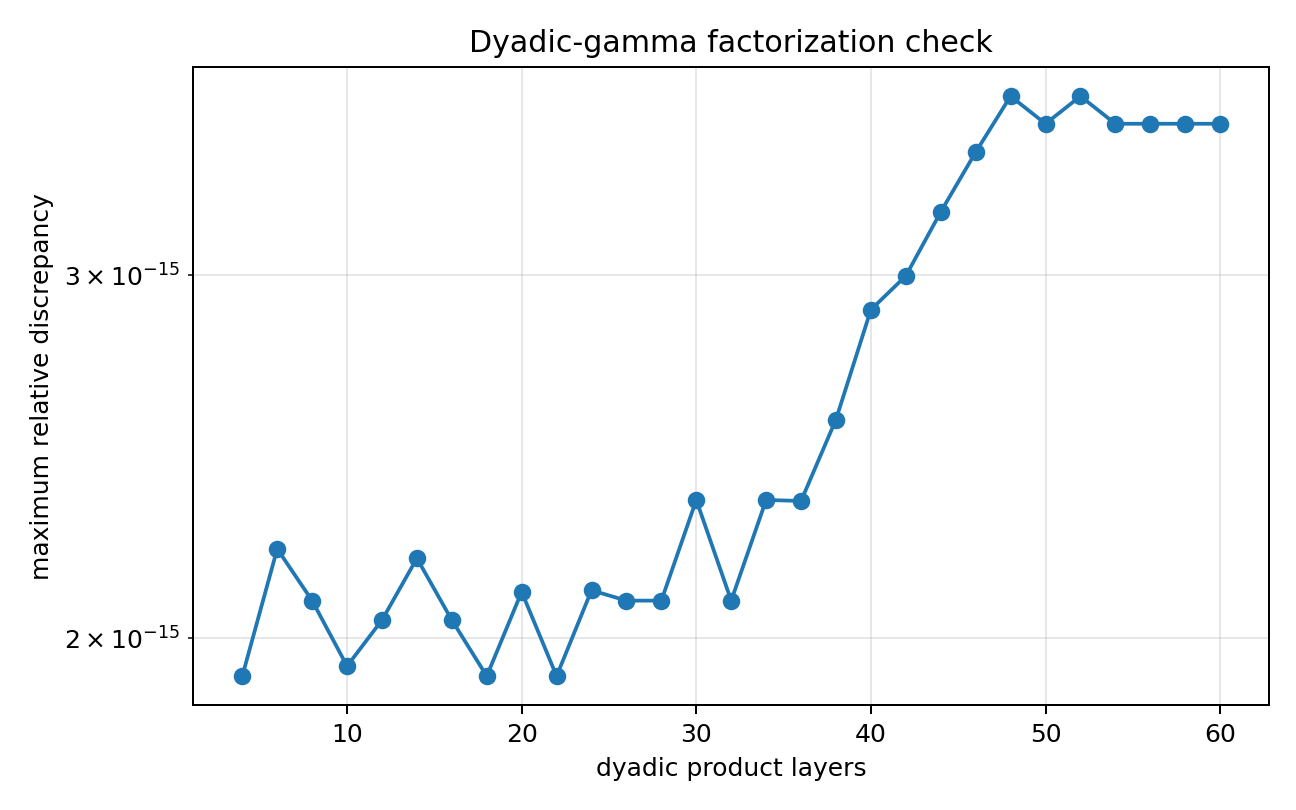
\includegraphics[width=0.78\textwidth]{figures/gamma_factorization_convergence.png}
\caption{Finite-layer check of the dyadic-gamma reflection factorization.}
\label{fig:gamma-check}
\end{figure}

\subsection{Jensen mean}

Angular trapezoidal quadrature with $8192$ nodes was compared with the exact zero-divisor
formula on $76$ radii.  The maximum absolute discrepancy was
$7.11\times10^{-15}$.  Representative values are
\begin{center}
\begin{tabular}{@{}rrrr@{}}
\toprule
$r$ & angular quadrature & exact formula & error \\
\midrule
$0.6$ & $-3.6082\times10^{-16}$ & $0$ & $-3.61\times10^{-16}$ \\
$1.4$ & $0.6729444732424255$ & $0.6729444732424258$ & $-3.33\times10^{-16}$ \\
$3.7$ & $5.496849257625430$ & $5.496849257625430$ & $0$ \\
$10.3$ & $26.15154490220755$ & $26.15154490220754$ & $3.55\times10^{-15}$ \\
\bottomrule
\end{tabular}
\end{center}

\begin{figure}[H]
\centering
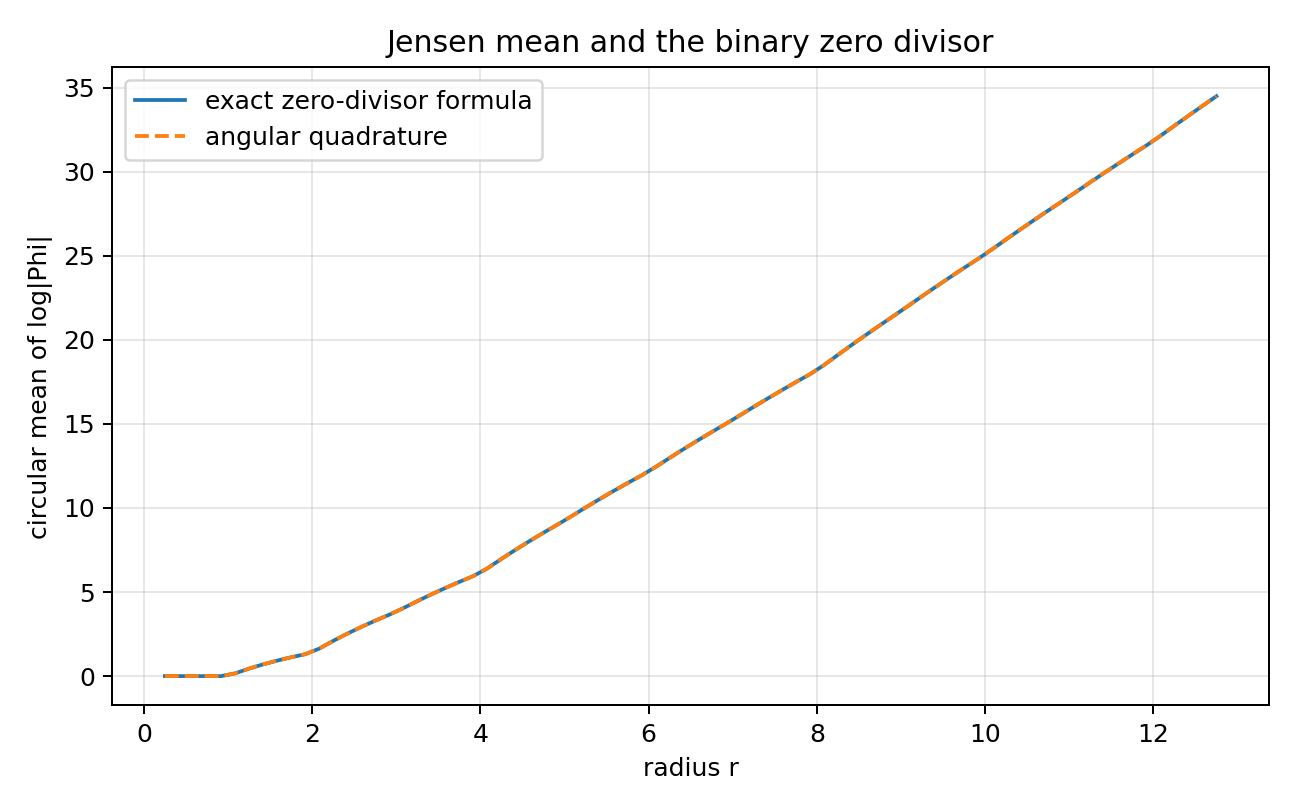
\includegraphics[width=0.78\textwidth]{figures/jensen_mean_comparison.png}
\caption{Jensen's angular mean versus the exact factorial/zero-divisor expression.}
\label{fig:jensen-check}
\end{figure}

\subsection{Logistic series versus Gaussian mixture}

The simulation used $100{,}000$ samples.  The logistic series retained sixteen dyadic layers;
its omitted standard deviation was $5.09\times10^{-6}$.  The gamma mixture retained the first
$250$ spectral sites and added the exact mean of the positive tail.  The tail standard
deviation was $2.07\times10^{-4}$, negligible compared with the exact standard deviation
$1/3$ of $Z_1$.  The two-sample Kolmogorov--Smirnov statistic was $0.00347$ with p-value
$0.5825$.  Sample variances were $0.1114725$ and $0.1110627$, compared with the exact
$1/9=0.1111111\ldots$.

\begin{figure}[H]
\centering
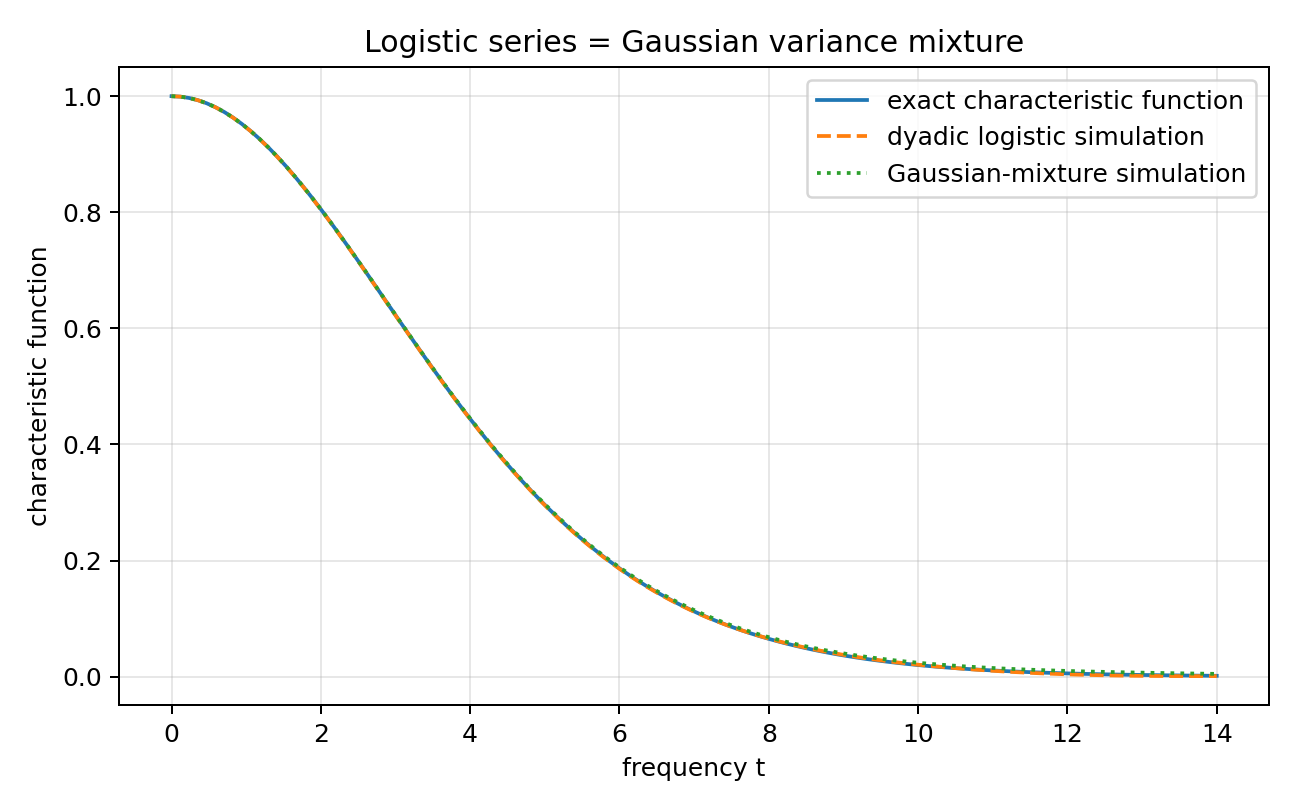
\includegraphics[width=0.78\textwidth]{figures/gaussian_mixture_characteristic_function.png}
\caption{The exact characteristic function and two independent simulations of the law in
\eqref{eq:logistic-mixture-law}.}
\label{fig:mixture-check}
\end{figure}

\subsection{Fabius sine series}

The series \eqref{eq:F-sine-series} was compared with the independent Fourier integral
\eqref{eq:F-sine-integral}.  At $x=0.25$, for example,
\[
 F(0.25)=0.06944444445136150\quad\text{(integral)},
 \qquad
 0.06944444444444434\quad\text{(128 harmonics)}.
\]
The discrepancy is governed by the numerical quadrature floor after roughly thirty-two
harmonics.  The rapid early convergence is visible in \cref{fig:F-series-check}.

\begin{figure}[H]
\centering
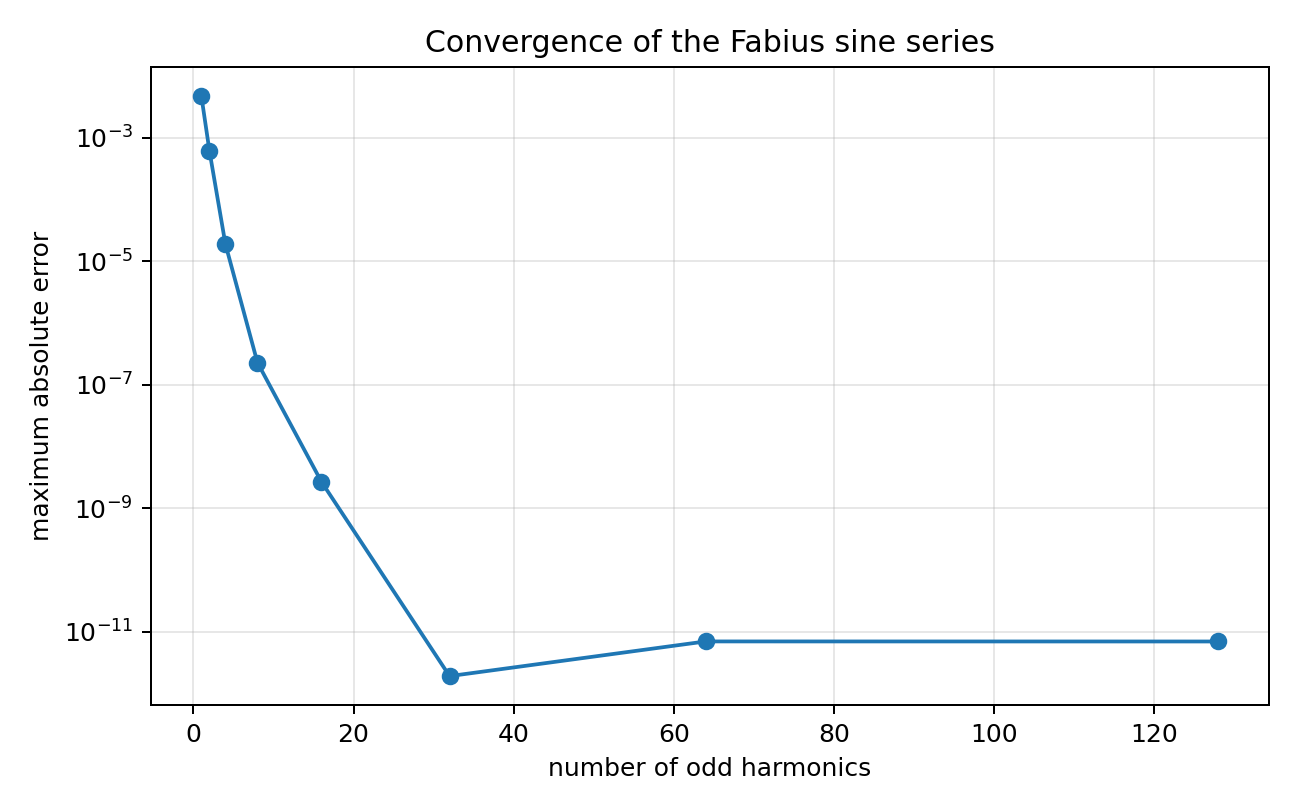
\includegraphics[width=0.78\textwidth]{figures/fabius_sine_series_convergence.png}
\caption{Maximum error of the odd-harmonic Fabius series against Fourier inversion on ten
sample points.}
\label{fig:F-series-check}
\end{figure}

\subsection{Reproduction command}

From the extracted package directory, run
\begin{lstlisting}[style=pythonstyle]
python numerical_experiments.py
\end{lstlisting}
The script creates no hidden cache and writes all outputs beneath \texttt{figures/}.  The
source comments explain the product truncations, gamma-tail correction, and quadrature
splitting at integer zeros.

\section{Conjectures and testable frontier statements}
\label{sec:conjectures}

\begin{conjecture}[Differential transcendence of the Fourier determinant \Conj]
The functions $\Phi$, $G_{\mathrm{dy}}$, and $\GammaDy$ are differentially transcendental
over $\C(z)$: none satisfies a nonzero algebraic differential equation with coefficients in
$\C(z)$.
\end{conjecture}

The non-D-finite theorem is evidence but does not approach the full differential-algebraic
claim.  A promising route is to combine the Mahler equation
\eqref{eq:GammaDy-Mahler} with differential Galois theory for mixed differential--difference
systems and the nonperiodic pole multiplicities.

\begin{conjecture}[Full Delange expansion of the Jensen mean \Conj]
There exist explicit continuous one-periodic functions $P_1,P_0$ such that
\begin{equation}
 J(r)=4r-\frac{(\log r)^2}{2\log2}
      +(\log r)P_1(\log_2r)+P_0(\log_2r)+\smallo(1),      \label{eq:J-Delange-conj}
\end{equation}
away from a controlled boundary layer around the integers.  The functions should be
computable from the Delange Fourier series for the binary digit sum and from the fractional
part $r-\floor r$.
\end{conjecture}

\begin{conjecture}[Asymptotics of inverse Fourier coefficients \Conj]
Let $c_n$ be defined by \eqref{eq:Q-sine-coeff}.  Then there is a bounded, nonconstant,
phase-dependent function $P$ such that
\begin{equation}
 \pi n c_n
 =Q(1/n)\left(P(\log_2\lambda_n)+\smallo(1)\right),      \label{eq:cn-conj}
\end{equation}
where $\lambda_n$ is the exact lower-Lambert saddle phase for $F(1/n)$.  In particular,
$\log|nc_n|$ should have leading scale
$-\sqrt{2\log2\,\log n}$ with the same periodic modulation that governs the inverse endpoint.
\end{conjecture}

This statement is testable by computing the oscillatory integral in
\eqref{eq:Q-sine-coeff} with the repository's certified endpoint saddle machinery.  It would
turn the local inverse asymptotic into a global spectral law for $Q$.

\begin{conjecture}[Hyperbolic complete monotonicity of the mixture density \Conj]
For every $\tau>0$, the function $s\mapsto p_\tau(\sqrt s)$ is hyperbolically completely
monotone, not merely completely monotone.  Equivalently, the normal variance mixture may lie
in the Bondesson class with a stronger multiplicative total-positivity structure inherited
from the discrete Thorin measure.
\end{conjecture}

\begin{conjecture}[Arithmetic special values of the dyadic gamma function \Conj]
At rational arguments with odd denominator, suitable products of
$\GammaDy(r)$, powers of $2\pi$, and classical Barnes multiple-gamma constants reduce to a
finite family of dyadic $L$-values and logarithmic $q$-products.  The functional equation
\eqref{eq:GammaDy-Mahler} should produce explicit distribution relations indexed by the
binary orbit of $r$.
\end{conjecture}

\begin{conjecture}[Optimal rational approximation from the Stieltjes resolvent \Conj]
Diagonal Pad\'e approximants obtained from
\(
 \Psi_{\mathrm{dy}}(-z)-\Psi_{\mathrm{dy}}(z)
\)
provide alternating, globally sharp rational bounds for $\Phi(\ii y)$ and for the
characteristic function of $Z_\tau$ on $y>0$, with error constants controlled explicitly by
the next unused spectral atom.
\end{conjecture}

\section{Promising research directions}
\label{sec:future}

\subsection{Formalization roadmap}

The shortest Lean route to the new results is modular.
\begin{enumerate}[leftmargin=2.3em]
\item Define $\GammaDy$ as a normally convergent product of meromorphic gamma factors and
      prove \eqref{eq:GammaDy-Mahler} and \eqref{eq:Phi-GammaDy} by the existing infinite
      product API.
\item Reuse the formal zero-multiplicity theorem to prove non-D-finiteness in a small
      analytic-ODE module.
\item Build $Z_\tau$ by conditioning a standard Gaussian on the already developed
      $V_\tau$, then identify characteristic functions.
\item Formalize Jensen's formula for the canonical product, followed by the finite factorial
      regrouping.  The digit-sum derivative then becomes arithmetic simplification.
\item Derive the compact and distributional Fourier transforms of $F$ from the existing
      transform of $\Up$ and a formal Heaviside distribution library.
\item Use the support-free quantile theorem and bounded-variation Fourier convergence to
      formalize \eqref{eq:Q-transform-nonlinear} and \eqref{eq:Q-sine-series}.
\end{enumerate}

\subsection{Spectral geometry and complex analysis}

The exact Jensen mean suggests treating $\Phi$ as an arithmetic spectral determinant in the
complex plane, not only on the real axis.  Natural next objects include logarithmic capacity,
angular large deviations of $\log|\Phi|$, Nevanlinna characteristics refined by binary digit
sums, and de Branges spaces generated by the reflected factors
$G_{\mathrm{dy}}(z)$ and $G_{\mathrm{dy}}(-z)$.

\subsection{Probability and semigroups}

The family $Z_\tau$ gives a canonical subordinate-Brownian semigroup attached to the Rvachev
zero divisor.  Its transition density, fractional generator, entropy production, and small-
time scaling should be expressible through the two heat kernels $L_1$ and $K$.  The explicit
Levy density \eqref{eq:Z-Levy-density} makes simulation, self-decomposability, and potential
theory accessible without reconstructing the gamma series term by term.

\subsection{Base-\texorpdfstring{$b$}{b} and geometric-\texorpdfstring{$q$}{q} families}

The geometric gamma factorization \eqref{eq:q-gamma-reflection} should be developed in
parallel with the repository's base-generic Gaussian-binomial interpolation.  For integer
$b$, the collision multiplicity of gamma poles is a whole-base valuation; for nonintegral
$q^{-1}$, the pole orbits are typically noncoincident.  Comparing these regimes may separate
which phenomena are genuinely dyadic from those caused only by geometric scaling.

\subsection{Inverse spectral analysis}

The coefficients \eqref{eq:Q-sine-coeff} provide a concrete meeting point for global Fourier
analysis and endpoint Lambert asymptotics.  Certified steepest-descent evaluation of these
coefficients could reveal periodic modulation, sign patterns, and optimal approximation
rates for the inverse.  A parallel study of
\(
 \int_0^1\e^{-2\pi\ii\eta F(x)}\dd x
\)
would produce a nonlinear Fourier theory of the CDF itself.

\subsection{Computer-assisted certification}

The existing Python checks are exploratory.  A rigorous package should combine interval
arithmetic for gamma products, exact rational moment recurrences, certified quadrature split
at the integer zero set, and explicit tail bounds from the rapid Fourier decay.  Such a tool
could test the conjectural Jensen fluctuation and inverse-coefficient phases at hundreds of
dyadic scales without confusing truncation error with genuine periodic oscillation.

\section{Conclusion}

The Fabius--Rvachev system is unusually rich because the same object can be read as a smooth
compact bump, a CDF, an infinite uniform convolution, a Thue--Morse spline limit, an entire
sinc determinant, an arithmetic spectrum, a $q$-series, and a Lambert-saddle problem.  The
source audit shows that many attractive formulae already coexist in the repository; treating
them as separate discoveries would obscure rather than advance the subject.

The new results in this report add bridges rather than isolated identities.  The dyadic gamma
function splits the even Fourier determinant into reflected arithmetic gamma factors.  The
Gaussian-mixture theorem joins the logistic/Appell dual to the Thorin/gamma dual and exposes a
new Levy semigroup.  Jensen's formula turns binary digit sums into a radial complex-analytic
observable.  Unbounded multiplicities settle non-holonomicity in one stroke.  Finally, the
bounded CDF and its inverse acquire transform formulae that are global, explicit, and
compatible with the existing endpoint theory.  Each bridge supplies both a theorem and a
research program, with a comparatively short path to formal verification.

\appendix

\section{Audited living document families}
\label{app:sources}

The active draft root at the audited snapshot contained the following document families.
Their exact names are retained to make future collision searches reproducible.

\begingroup
\small
\begin{longtable}{@{}p{0.39\textwidth}p{0.55\textwidth}@{}}
\toprule
Draft family & Principal audited themes \\
\midrule
\endfirsthead
\toprule
Draft family & Principal audited themes \\
\midrule
\endhead
\path{Fabius_Arithmetic_Rays_Frontier_Report} & arithmetic rays, exact values, spectral sampling \\
\path{Fabius_Dyadic_Self_Sampling_Frontier_Package} & dyadic self-sampling and reconstruction \\
\path{Fabius_Half_Integer_Spectral_Frontier_Report} & half-integer cosine spectrum, Prouhet identities, alias transforms \\
\path{Fabius_Inverse_Frontier_Report_Source_and_PDF} & inverse germs, Catalan and Lambert--Bell asymptotics \\
\path{Fabius_Newton_Rvachev_Frontier_Report} & Newton recurrences, exponent sequences, exact FFT checks \\
\path{Fabius_Rvachev_Frontier_Report-2} & arithmetic spectrum, zero multiplicities, heat trace, lobe signs \\
\path{Fabius_Rvachev_Frontier_Report} & tail quadrature, exact dyadic error laws, $q$-Richardson acceleration \\
\path{Fabius_Rvachev_New_Frontiers} & $q$-MZV moments, Thorin dual, complete Bernstein theory, theta completion \\
\path{Fabius_Rvachev_Thue_Morse_Frontier_Results} & finite blocks, deconvolution, zeta--Lambert tails \\
\path{Spectral_Arithmetic_Pascal_Rvachev_Hierarchy} & spectral arithmetic and Pascal-type hierarchies \\
\path{Thue_Morse_Formula_Atlas} & broad Thue--Morse product, series, automata, and arithmetic atlas \\
\path{fabius_frontier_dyadic_inverse_barnes_report} & dyadic inverse, Barnes prefixes, Appell and logistic dual \\
\path{fabius_frontier_new_results} & logarithmic $q$-Richardson and Lambert phase locking \\
\path{fabius_frontier_results} & $q$-Richardson sinc products and acceleration \\
\path{fabius_frontier_results_bundle} & Fredholm determinant, spectral zeta, zero jets, $q$-Euler determinant \\
\path{fabius_frontier_spectral_endpoint_report_bundle} & endpoint spectral products, Mellin and saddle analysis \\
\path{rvachev_up_fourier_decay} & successive Fourier-decay audits and certified bounds \\
\bottomrule
\end{longtable}
\endgroup

The source audit also included the primary formal article, the consolidated
\texttt{non-formalized-}\allowbreak\texttt{research-frontiers.tex}, glossary, Lean walkthrough, non-elementarity
document, embedded papers, and the archive provenance map.  The archive map was essential for
identifying superseded or byte-identical historical variants without treating them as
independent sources.

\section{Numerical package contents}
\label{app:package}

The ZIP archive accompanying this report contains:
\begin{itemize}[leftmargin=2em]
\item \texttt{fabius\_rvachev\_representation\_frontier\_report.tex};
\item the compiled PDF with the same basename;
\item \texttt{numerical\_experiments.py}, with detailed comments and deterministic seed;
\item \texttt{figures/numerical\_results.txt};
\item the four PNG figures embedded in the report;
\item \texttt{SOURCE\_AUDIT.md}, a concise audit and novelty-collision record;
\item \texttt{README.md}, reproduction instructions and file descriptions.
\end{itemize}

\section{Selected derivations in one line}
\label{app:one-line}

For convenient reuse, here are the central bridges in compressed form:
\begin{align*}
 \Gamma(1+w)\Gamma(1-w)&=1/\sinc(\pi w)
 &&\Longrightarrow\quad \Phi(z)=1/[\GammaDy(z)\GammaDy(-z)],\\
 \E\e^{-wV_\tau}&=\Acal(w)^{-\tau},\quad
 \E(\e^{\ii t\sqrt{2T}N}\mid T)=\e^{-t^2T}
 &&\Longrightarrow\quad Z_1\dist\sqrt{2T_1}N,\\
 \operatorname{zeros}(\Phi)&=\{\pm n\text{ with multiplicity }a_n\}
 &&\Longrightarrow\quad J(r)=2\sum_{n\le r}a_n\log(r/n),\\
 a_{2^k}&=k+1\to\infty
 &&\Longrightarrow\quad \Phi\text{ is not D-finite},\\
 F'(x)&=2\Up(2x-1),\quad \widehat\Up=\Phi
 &&\Longrightarrow\quad \widehat{F'}(\xi)=\e^{-\pi\ii\xi}\Phi(\xi/2),\\
 y&=F(x),\quad Q(F(x))=x
 &&\Longrightarrow\quad
 \widehat Q(\eta)=\frac{\int_0^1\e^{-2\pi\ii\eta F(x)}\dd x-
 \e^{-2\pi\ii\eta}}{2\pi\ii\eta}.
\end{align*}

\begin{thebibliography}{99}

\bibitem{jessen1935}
B.~Jessen and A.~Wintner,
\newblock Distribution functions and the Riemann zeta function,
\newblock \emph{Transactions of the American Mathematical Society}
\textbf{38} (1935), 48--88.

\bibitem{fabius1966}
J.~Fabius,
\newblock A probabilistic example of a nowhere analytic $C^\infty$-function,
\newblock \emph{Zeitschrift f\"ur Wahrscheinlichkeitstheorie und Verwandte Gebiete}
\textbf{5} (1966), 173--174.
\newblock DOI: \nolinkurl{10.1007/BF00536652}.

\bibitem{rvachev1971}
V.~L.~Rvachev and V.~A.~Rvachev,
\newblock A certain finite function,
\newblock \emph{Dopovidi Akademii Nauk Ukrains'koi RSR, Series A}
(1971), 705--707, 764.

\bibitem{rvachev1990}
V.~A.~Rvachev,
\newblock Compactly supported solutions of functional-differential equations and their
applications,
\newblock \emph{Russian Mathematical Surveys} \textbf{45} (1990), no.~1, 87--120.

\bibitem{arias1982}
J.~Arias de Reyna,
\newblock Definici\'on y estudio de una funci\'on indefinidamente diferenciable de soporte
compacto,
\newblock \emph{Revista de la Real Academia de Ciencias Exactas, F\'isicas y Naturales de
Madrid} \textbf{76} (1982), no.~1, 21--38.
\newblock English translation: \emph{An infinitely differentiable function with compact
support: Definition and properties}, arXiv:1702.05442 (2017).

\bibitem{arias2018}
J.~Arias de Reyna,
\newblock Arithmetic of the Fabius function,
\newblock \emph{INTEGERS} \textbf{18} (2018), Article A51; arXiv:1702.06487, version~3.

\bibitem{haugland2016}
J.~K.~Haugland,
\newblock Evaluating the Fabius function,
\newblock arXiv:1609.07999 (2016).

\bibitem{allouche2003}
J.-P.~Allouche and J.~Shallit,
\newblock \emph{Automatic Sequences: Theory, Applications, Generalizations},
\newblock Cambridge University Press, 2003.

\bibitem{corless1996}
R.~M.~Corless, G.~H.~Gonnet, D.~E.~G.~Hare, D.~J.~Jeffrey, and D.~E.~Knuth,
\newblock On the Lambert $W$ function,
\newblock \emph{Advances in Computational Mathematics} \textbf{5} (1996), 329--359.

\bibitem{flajolet1995}
P.~Flajolet, X.~Gourdon, and P.~Dumas,
\newblock Mellin transforms and asymptotics: harmonic sums,
\newblock \emph{Theoretical Computer Science} \textbf{144} (1995), 3--58.

\bibitem{andrews1976}
G.~E.~Andrews,
\newblock \emph{The Theory of Partitions},
\newblock Addison--Wesley, 1976.

\bibitem{gasper2004}
G.~Gasper and M.~Rahman,
\newblock \emph{Basic Hypergeometric Series}, second edition,
\newblock Cambridge University Press, 2004.

\bibitem{bondesson1992}
L.~Bondesson,
\newblock \emph{Generalized Gamma Convolutions and Related Classes of Distributions and
Densities},
\newblock Lecture Notes in Statistics 76, Springer, 1992.

\bibitem{sato1999}
K.-I.~Sato,
\newblock \emph{L\'evy Processes and Infinitely Divisible Distributions},
\newblock Cambridge University Press, 1999.

\bibitem{schoenberg1938}
I.~J.~Schoenberg,
\newblock Metric spaces and completely monotone functions,
\newblock \emph{Annals of Mathematics} \textbf{39} (1938), 811--841.

\bibitem{stanley1980}
R.~P.~Stanley,
\newblock Differentiably finite power series,
\newblock \emph{European Journal of Combinatorics} \textbf{1} (1980), 175--188.

\bibitem{proveit}
V.~Reshetnikov,
\newblock \emph{ProveIt: Analysis/FabiusFunction},
\newblock Lean~4 formal development and document corpus, source snapshot
\CommitID, consulted 27 August 2026.
\newblock \url{https://github.com/VladimirReshetnikov/ProveIt/tree/0770442945d65bac5530c4f214c6c52c4cb9fbdc/Analysis/FabiusFunction}.

\end{thebibliography}

\end{document}
